\PassOptionsToPackage{unicode=true}{hyperref} % options for packages loaded elsewhere
\PassOptionsToPackage{hyphens}{url}
\PassOptionsToPackage{dvipsnames,svgnames*,x11names*}{xcolor}
%
\documentclass[ignorenonframetext,]{beamer}
\usepackage{pgfpages}
\setbeamertemplate{caption}[numbered]
\setbeamertemplate{caption label separator}{: }
\setbeamercolor{caption name}{fg=normal text.fg}
\beamertemplatenavigationsymbolsempty
\usepackage{lmodern}
\usepackage{amssymb,amsmath}
\usepackage{ifxetex,ifluatex}
\usepackage{fixltx2e} % provides \textsubscript
\ifnum 0\ifxetex 1\fi\ifluatex 1\fi=0 % if pdftex
  \usepackage[T1]{fontenc}
  \usepackage[utf8]{inputenc}
  \usepackage{textcomp} % provides euro and other symbols
\else % if luatex or xelatex
  \usepackage{unicode-math}
  \defaultfontfeatures{Ligatures=TeX,Scale=MatchLowercase}
\fi
% use upquote if available, for straight quotes in verbatim environments
\IfFileExists{upquote.sty}{\usepackage{upquote}}{}
% use microtype if available
\IfFileExists{microtype.sty}{%
\usepackage[]{microtype}
\UseMicrotypeSet[protrusion]{basicmath} % disable protrusion for tt fonts
}{}
\IfFileExists{parskip.sty}{%
\usepackage{parskip}
}{% else
\setlength{\parindent}{0pt}
\setlength{\parskip}{6pt plus 2pt minus 1pt}
}
\usepackage{xcolor}
\usepackage{hyperref}
\hypersetup{
            pdftitle={Reproducible (and collaborative) science through RStudio},
            pdfauthor={Jenny Rieck \& Derek Beaton},
            colorlinks=true,
            linkcolor=Maroon,
            citecolor=Blue,
            urlcolor=blue,
            breaklinks=true}
\urlstyle{same}  % don't use monospace font for urls
\newif\ifbibliography
\usepackage{color}
\usepackage{fancyvrb}
\newcommand{\VerbBar}{|}
\newcommand{\VERB}{\Verb[commandchars=\\\{\}]}
\DefineVerbatimEnvironment{Highlighting}{Verbatim}{commandchars=\\\{\}}
% Add ',fontsize=\small' for more characters per line
\usepackage{framed}
\definecolor{shadecolor}{RGB}{248,248,248}
\newenvironment{Shaded}{\begin{snugshade}}{\end{snugshade}}
\newcommand{\AlertTok}[1]{\textcolor[rgb]{0.94,0.16,0.16}{#1}}
\newcommand{\AnnotationTok}[1]{\textcolor[rgb]{0.56,0.35,0.01}{\textbf{\textit{#1}}}}
\newcommand{\AttributeTok}[1]{\textcolor[rgb]{0.77,0.63,0.00}{#1}}
\newcommand{\BaseNTok}[1]{\textcolor[rgb]{0.00,0.00,0.81}{#1}}
\newcommand{\BuiltInTok}[1]{#1}
\newcommand{\CharTok}[1]{\textcolor[rgb]{0.31,0.60,0.02}{#1}}
\newcommand{\CommentTok}[1]{\textcolor[rgb]{0.56,0.35,0.01}{\textit{#1}}}
\newcommand{\CommentVarTok}[1]{\textcolor[rgb]{0.56,0.35,0.01}{\textbf{\textit{#1}}}}
\newcommand{\ConstantTok}[1]{\textcolor[rgb]{0.00,0.00,0.00}{#1}}
\newcommand{\ControlFlowTok}[1]{\textcolor[rgb]{0.13,0.29,0.53}{\textbf{#1}}}
\newcommand{\DataTypeTok}[1]{\textcolor[rgb]{0.13,0.29,0.53}{#1}}
\newcommand{\DecValTok}[1]{\textcolor[rgb]{0.00,0.00,0.81}{#1}}
\newcommand{\DocumentationTok}[1]{\textcolor[rgb]{0.56,0.35,0.01}{\textbf{\textit{#1}}}}
\newcommand{\ErrorTok}[1]{\textcolor[rgb]{0.64,0.00,0.00}{\textbf{#1}}}
\newcommand{\ExtensionTok}[1]{#1}
\newcommand{\FloatTok}[1]{\textcolor[rgb]{0.00,0.00,0.81}{#1}}
\newcommand{\FunctionTok}[1]{\textcolor[rgb]{0.00,0.00,0.00}{#1}}
\newcommand{\ImportTok}[1]{#1}
\newcommand{\InformationTok}[1]{\textcolor[rgb]{0.56,0.35,0.01}{\textbf{\textit{#1}}}}
\newcommand{\KeywordTok}[1]{\textcolor[rgb]{0.13,0.29,0.53}{\textbf{#1}}}
\newcommand{\NormalTok}[1]{#1}
\newcommand{\OperatorTok}[1]{\textcolor[rgb]{0.81,0.36,0.00}{\textbf{#1}}}
\newcommand{\OtherTok}[1]{\textcolor[rgb]{0.56,0.35,0.01}{#1}}
\newcommand{\PreprocessorTok}[1]{\textcolor[rgb]{0.56,0.35,0.01}{\textit{#1}}}
\newcommand{\RegionMarkerTok}[1]{#1}
\newcommand{\SpecialCharTok}[1]{\textcolor[rgb]{0.00,0.00,0.00}{#1}}
\newcommand{\SpecialStringTok}[1]{\textcolor[rgb]{0.31,0.60,0.02}{#1}}
\newcommand{\StringTok}[1]{\textcolor[rgb]{0.31,0.60,0.02}{#1}}
\newcommand{\VariableTok}[1]{\textcolor[rgb]{0.00,0.00,0.00}{#1}}
\newcommand{\VerbatimStringTok}[1]{\textcolor[rgb]{0.31,0.60,0.02}{#1}}
\newcommand{\WarningTok}[1]{\textcolor[rgb]{0.56,0.35,0.01}{\textbf{\textit{#1}}}}
\usepackage{graphicx,grffile}
\makeatletter
\def\maxwidth{\ifdim\Gin@nat@width>\linewidth\linewidth\else\Gin@nat@width\fi}
\def\maxheight{\ifdim\Gin@nat@height>\textheight\textheight\else\Gin@nat@height\fi}
\makeatother
% Scale images if necessary, so that they will not overflow the page
% margins by default, and it is still possible to overwrite the defaults
% using explicit options in \includegraphics[width, height, ...]{}
\setkeys{Gin}{width=\maxwidth,height=\maxheight,keepaspectratio}
% Prevent slide breaks in the middle of a paragraph:
\widowpenalties 1 10000
\raggedbottom
\setbeamertemplate{part page}{
\centering
\begin{beamercolorbox}[sep=16pt,center]{part title}
  \usebeamerfont{part title}\insertpart\par
\end{beamercolorbox}
}
\setbeamertemplate{section page}{
\centering
\begin{beamercolorbox}[sep=12pt,center]{part title}
  \usebeamerfont{section title}\insertsection\par
\end{beamercolorbox}
}
\setbeamertemplate{subsection page}{
\centering
\begin{beamercolorbox}[sep=8pt,center]{part title}
  \usebeamerfont{subsection title}\insertsubsection\par
\end{beamercolorbox}
}
\AtBeginPart{
  \frame{\partpage}
}
\AtBeginSection{
  \ifbibliography
  \else
    \frame{\sectionpage}
  \fi
}
\AtBeginSubsection{
  \frame{\subsectionpage}
}
\setlength{\emergencystretch}{3em}  % prevent overfull lines
\providecommand{\tightlist}{%
  \setlength{\itemsep}{0pt}\setlength{\parskip}{0pt}}
\setcounter{secnumdepth}{0}

% set default figure placement to htbp
\makeatletter
\def\fps@figure{htbp}
\makeatother


\title{Reproducible (and collaborative) science through RStudio}
\providecommand{\subtitle}[1]{}
\subtitle{A whirlwind tour with R, RMarkdown, Python, LaTeX, and more}
\author{Jenny Rieck \& Derek Beaton}
\date{May 22 2019}

\begin{document}
\frame{\titlepage}

\begin{frame}{The big outline}
\protect\hypertarget{the-big-outline}{}

\begin{itemize}
\tightlist
\item
  Part 0: Background
\item
  Part 1: A bit about R
\item
  Part 2: RStudio \& Project setup
\item
  Part 3: R
\item
  Part 4: RMarkdown \& more
\item
  Part 5: ``Advanced'' topics
\end{itemize}

\end{frame}

\hypertarget{part-0-background}{%
\section{Part 0: Background}\label{part-0-background}}

\begin{frame}{To dive right in}
\protect\hypertarget{to-dive-right-in}{}

If you want to skip over the background \& RStudio, go straight to
\protect\hyperlink{part-2-rstudio-project-setup}{Part 2: RStudio \&
Project setup}

\end{frame}

\begin{frame}[fragile]{Background}
\protect\hypertarget{background}{}

\begin{itemize}
\tightlist
\item
  This is a taste and to bring you into a bigger world

  \begin{itemize}
  \tightlist
  \item
    R, Python, SQL, and JavaScript are critical data science
    tools/languages
  \end{itemize}
\item
  R (language and community) strongly emphasizes

  \begin{itemize}
  \tightlist
  \item
    Centralization \& standards
  \item
    Rigor \& reproducibility (packages, RMarkdown)
  \item
    An interesting language
  \end{itemize}
\item
  Functional

  \begin{itemize}
  \tightlist
  \item
    With a sublanguage (or dialect?): the \texttt{tidyverse}
  \end{itemize}
\end{itemize}

\end{frame}

\begin{frame}{R is a community (actually many communities!)}
\protect\hypertarget{r-is-a-community-actually-many-communities}{}

\begin{itemize}
\tightlist
\item
  Help and resources
\item
  Package development and distribution
\item
  An ideal example

  \begin{itemize}
  \tightlist
  \item
    Not quite always that way
  \item
    Strong communal presence
  \end{itemize}
\end{itemize}

\end{frame}

\begin{frame}{R: Help!}
\protect\hypertarget{r-help}{}

\begin{itemize}
\tightlist
\item
  So many websites e.g., \url{https://www.statmethods.net/}
\item
  Online forums (Stack Exchange, r-lists)
\item
  SpringerLink

  \begin{itemize}
  \tightlist
  \item
    All R books for free (pdf format) or for minimal cost (printed)
  \end{itemize}
\item
  Vignettes

  \begin{itemize}
  \tightlist
  \item
    step-by-step instruction guides for packages
  \end{itemize}
\item
  Git

  \begin{itemize}
  \tightlist
  \item
    With open books (via bookdown)
  \end{itemize}
\item
  Twitter \#rstats
\item
  RStudio (website)

  \begin{itemize}
  \tightlist
  \item
    Videos, cheat sheets
  \end{itemize}
\end{itemize}

\end{frame}

\begin{frame}{R Packages}
\protect\hypertarget{r-packages}{}

\begin{itemize}
\tightlist
\item
  Packages are bundles of code made by someone (or many people) for
  everyone to use
\item
  There are packages for everything
\item
  We'll cover some of the diversity throughout
\item
  Comprehensive \& Reproducible

  \begin{itemize}
  \tightlist
  \item
    Available primarily on CRAN
  \item
    But also github (less so: r-forge)
  \end{itemize}
\end{itemize}

\end{frame}

\hypertarget{part-1-a-bit-about-r}{%
\section{Part 1: A bit about R}\label{part-1-a-bit-about-r}}

\begin{frame}{R Background}
\protect\hypertarget{r-background}{}

\begin{itemize}
\tightlist
\item
  Created in 1992 by Gentleman \& Ihaka
\end{itemize}

\emph{{[}we{]} considered the problem of obtaining decent statistical
software for our undergraduate Macintosh lab. After considering the
options, we decided that the most satisfactory alternative was to write
our own. {[}\ldots{}{]} Finally we added some syntactic sugar to make it
look somewhat like S. We call the result ``R''.}

\end{frame}

\begin{frame}{What is R?}
\protect\hypertarget{what-is-r}{}

\begin{itemize}
\tightlist
\item
  R is general purpose programming

  \begin{itemize}
  \tightlist
  \item
    Design around \& for statistics
  \item
    ``for and by statisticians''
  \end{itemize}
\item
  R is a collection of tools

  \begin{itemize}
  \tightlist
  \item
    Pre-packaged software at your disposal
  \end{itemize}
\item
  R is free (as in beer and speech)

  \begin{itemize}
  \tightlist
  \item
    No cost, no restrictions
  \item
    E.g., Microsoft (nee Revolution) R
  \end{itemize}
\item
  R is a functional language

  \begin{itemize}
  \tightlist
  \item
    Turing complete
  \item
    Mathematical functions
  \item
    Pass expressions and functions to and from functions
  \end{itemize}
\end{itemize}

\end{frame}

\begin{frame}{Some syntax notes}
\protect\hypertarget{some-syntax-notes}{}

\end{frame}

\begin{frame}[fragile]{Assignment}
\protect\hypertarget{assignment}{}

\begin{Shaded}
\begin{Highlighting}[]
\CommentTok{# allowed but not preferred}
\NormalTok{a_variable =}\StringTok{ }\DecValTok{10} \OperatorTok{+}\StringTok{ }\DecValTok{1}
\CommentTok{# preferred}
\NormalTok{a_variable <-}\StringTok{ }\DecValTok{10} \OperatorTok{+}\StringTok{ }\DecValTok{1}
\CommentTok{# a bonus}
\DecValTok{10} \OperatorTok{+}\StringTok{ }\DecValTok{1}\NormalTok{ ->}\StringTok{ }\NormalTok{a_variable}
\end{Highlighting}
\end{Shaded}

\end{frame}

\begin{frame}[fragile]{Dots}
\protect\hypertarget{dots}{}

\begin{Shaded}
\begin{Highlighting}[]
\CommentTok{# allowed but not preferred}
\NormalTok{a.variable =}\StringTok{ }\DecValTok{10} \OperatorTok{+}\StringTok{ }\DecValTok{1}
\NormalTok{  ## dots have 2 meanings in R, }
\NormalTok{    ## with a 3rd in the tidyverse}

\CommentTok{# preferred}
\NormalTok{a_variable <-}\StringTok{ }\DecValTok{10} \OperatorTok{+}\StringTok{ }\DecValTok{1}
\end{Highlighting}
\end{Shaded}

\end{frame}

\begin{frame}[fragile]{``Reserved'' characters}
\protect\hypertarget{reserved-characters}{}

\begin{itemize}
\tightlist
\item
  \texttt{c}, \texttt{q}, \texttt{t}, \texttt{C}, \texttt{D},
  \texttt{I}, \texttt{F}, and \texttt{T} (via
  \url{https://www.johndcook.com/blog/r_language_for_programmers/})
\item
  Except that these can be redefined

  \begin{itemize}
  \tightlist
  \item
    With great power comes great responsibility (and danger)
  \end{itemize}
\end{itemize}

\end{frame}

\begin{frame}[fragile]{R: Data types}
\protect\hypertarget{r-data-types}{}

\begin{itemize}
\tightlist
\item
  Stored as \emph{vectors}

  \begin{itemize}
  \tightlist
  \item
    see \texttt{class()}
  \end{itemize}
\item
  numeric

  \begin{itemize}
  \tightlist
  \item
    real or decimal
  \item
    Includes \texttt{NaN}, \texttt{Inf}, \texttt{-Inf}
  \end{itemize}
\item
  integer
\item
  complex
\item
  character
\item
  logical

  \begin{itemize}
  \tightlist
  \item
    includes \texttt{NA}, \texttt{TRUE}, \texttt{FALSE}
  \end{itemize}
\item
  factor

  \begin{itemize}
  \tightlist
  \item
    factors are usually not your friends
  \item
    with \texttt{read.csv()}: \texttt{stringsAsFactors\ =\ F} or convert
    these
  \item
    or use \texttt{tibble}s in the tidyverse
  \end{itemize}
\end{itemize}

\end{frame}

\begin{frame}[fragile]{R: factor disasters}
\protect\hypertarget{r-factor-disasters}{}

\begin{Shaded}
\begin{Highlighting}[]
\NormalTok{a_numeric_vector <-}\StringTok{ }\KeywordTok{c}\NormalTok{(}\DecValTok{3}\NormalTok{, }\DecValTok{0}\NormalTok{, }\DecValTok{1}\NormalTok{, }\DecValTok{-2}\NormalTok{, }\DecValTok{2}\NormalTok{, }\DecValTok{5}\NormalTok{, }\DecValTok{5}\NormalTok{, }\DecValTok{2}\NormalTok{, }\DecValTok{1}\NormalTok{)}
\NormalTok{(a_numeric_vector }\OperatorTok{+}\StringTok{ }\DecValTok{1}\NormalTok{)}
\end{Highlighting}
\end{Shaded}

\begin{verbatim}
## [1]  4  1  2 -1  3  6  6  3  2
\end{verbatim}

\begin{Shaded}
\begin{Highlighting}[]
\NormalTok{(a_numeric2factor_vector <-}\StringTok{ }\KeywordTok{as.factor}\NormalTok{(a_numeric_vector))}
\end{Highlighting}
\end{Shaded}

\begin{verbatim}
## [1] 3  0  1  -2 2  5  5  2  1 
## Levels: -2 0 1 2 3 5
\end{verbatim}

\begin{Shaded}
\begin{Highlighting}[]
\NormalTok{(}\KeywordTok{as.numeric}\NormalTok{(a_numeric2factor_vector))}
\end{Highlighting}
\end{Shaded}

\begin{verbatim}
## [1] 5 2 3 1 4 6 6 4 3
\end{verbatim}

\begin{Shaded}
\begin{Highlighting}[]
\NormalTok{(}\KeywordTok{as.numeric}\NormalTok{(}\KeywordTok{as.character}\NormalTok{(a_numeric2factor_vector)))}
\end{Highlighting}
\end{Shaded}

\begin{verbatim}
## [1]  3  0  1 -2  2  5  5  2  1
\end{verbatim}

\end{frame}

\begin{frame}[fragile]{R: Data structures}
\protect\hypertarget{r-data-structures}{}

\begin{itemize}
\tightlist
\item
  Starts counting from 1

  \begin{itemize}
  \tightlist
  \item
    Not 0
  \end{itemize}
\item
  vector{[}1{]}
\item
  matrix{[}1,1{]}
\item
  array{[}1,1,1{]}
\item
  list{[}{[}1{]}{]}

  \begin{itemize}
  \tightlist
  \item
    Can contain mixtures of types
  \item
    or list\$\texttt{name}
  \end{itemize}
\item
  data.frame:

  \begin{itemize}
  \tightlist
  \item
    Is technically a list but access in three ways
  \item
    data.frame{[}{[}1{]}{]}{[}1{]}
  \item
    data.frame{[}1,1{]}
  \item
    data.frame\$\texttt{name}
  \item
    tibbles: tidyverse data.frames
  \end{itemize}
\end{itemize}

\end{frame}

\begin{frame}{Cheatsheet for going from MatLab to R}
\protect\hypertarget{cheatsheet-for-going-from-matlab-to-r}{}

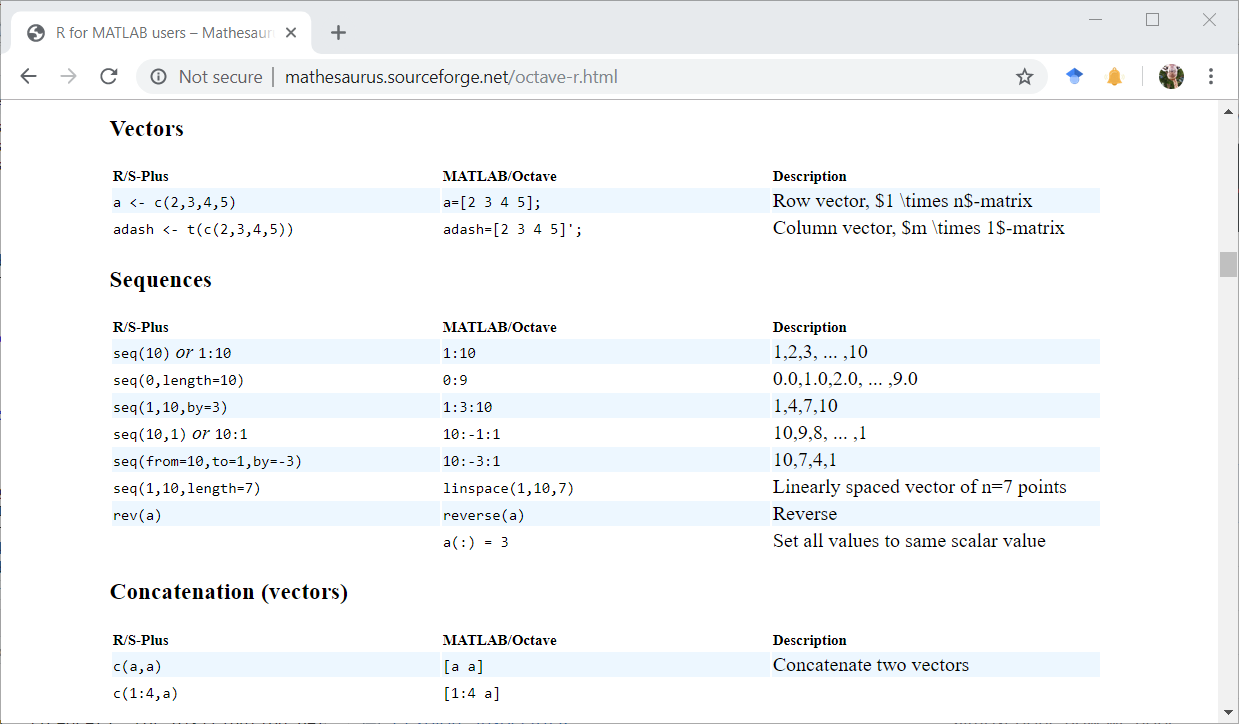
\includegraphics{../external/images/r_cheatsheet_matlab.PNG}
\url{http://mathesaurus.sourceforge.net/octave-r.html}

\end{frame}

\begin{frame}{Cheatsheet for base R}
\protect\hypertarget{cheatsheet-for-base-r}{}

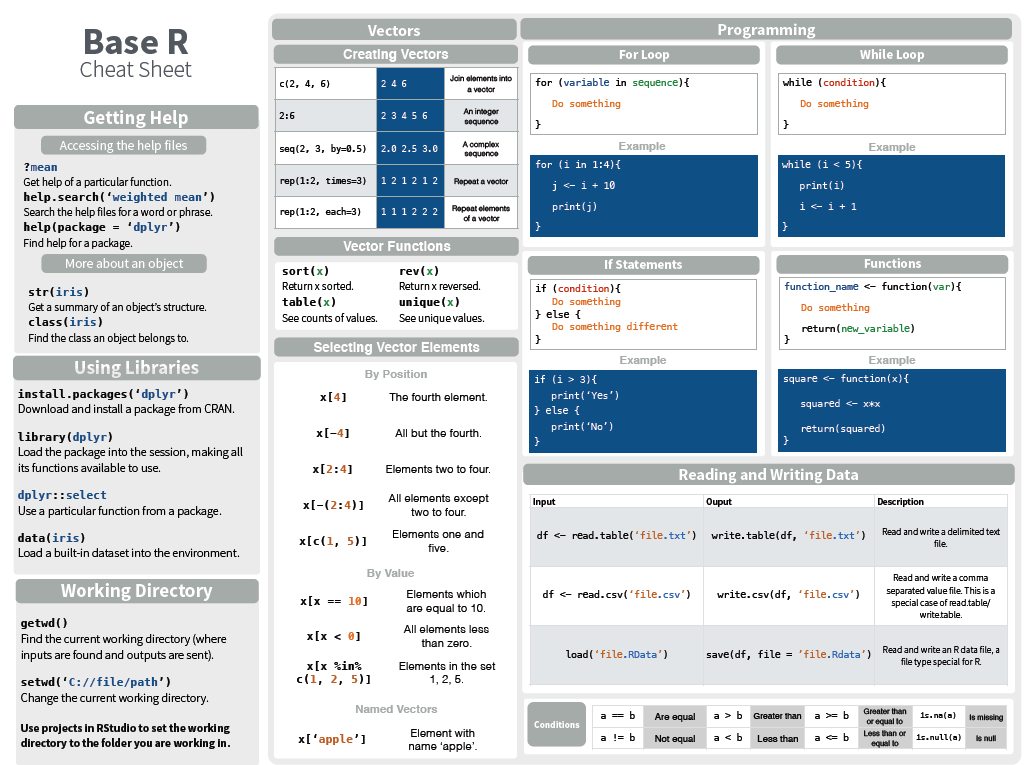
\includegraphics{../external/images/r_cheatsheet_base.PNG}

\end{frame}

\begin{frame}[fragile]{Tidyverse}
\protect\hypertarget{tidyverse}{}

\begin{itemize}
\tightlist
\item
  R is ``base R''
\item
  \texttt{tidyverse}: ``an opinionated collection of R packages designed
  for data science {[}that{]} share an underlying design philosophy,
  \textbf{grammar, and data structures.}''

  \begin{itemize}
  \tightlist
  \item
    Started(?) with/because of \texttt{ggplot2}
  \item
    A sublanguage or dialect
  \item
    Can do so because R is functional language
  \item
    For full tidy immersion see: \url{https://style.tidyverse.org/}
  \end{itemize}
\item
  Strongly built around a style:

  \begin{itemize}
  \tightlist
  \item
    objects are nouns
  \item
    functions are verbs
  \end{itemize}
\item
  Core packages:

  \begin{itemize}
  \tightlist
  \item
    \texttt{ggplot2}, \texttt{dplyr}, \texttt{tidyr}, \texttt{readr},
    \texttt{tibble}, \texttt{stringr}
  \end{itemize}
\item
  Get them all with \texttt{install.packages("tidyverse")}
\item
  Learn it!

  \begin{itemize}
  \tightlist
  \item
    But don't learn \emph{only} the tidyverse, you'll be lost in base R
  \end{itemize}
\end{itemize}

\end{frame}

\begin{frame}{tidyverse cheatsheet}
\protect\hypertarget{tidyverse-cheatsheet}{}

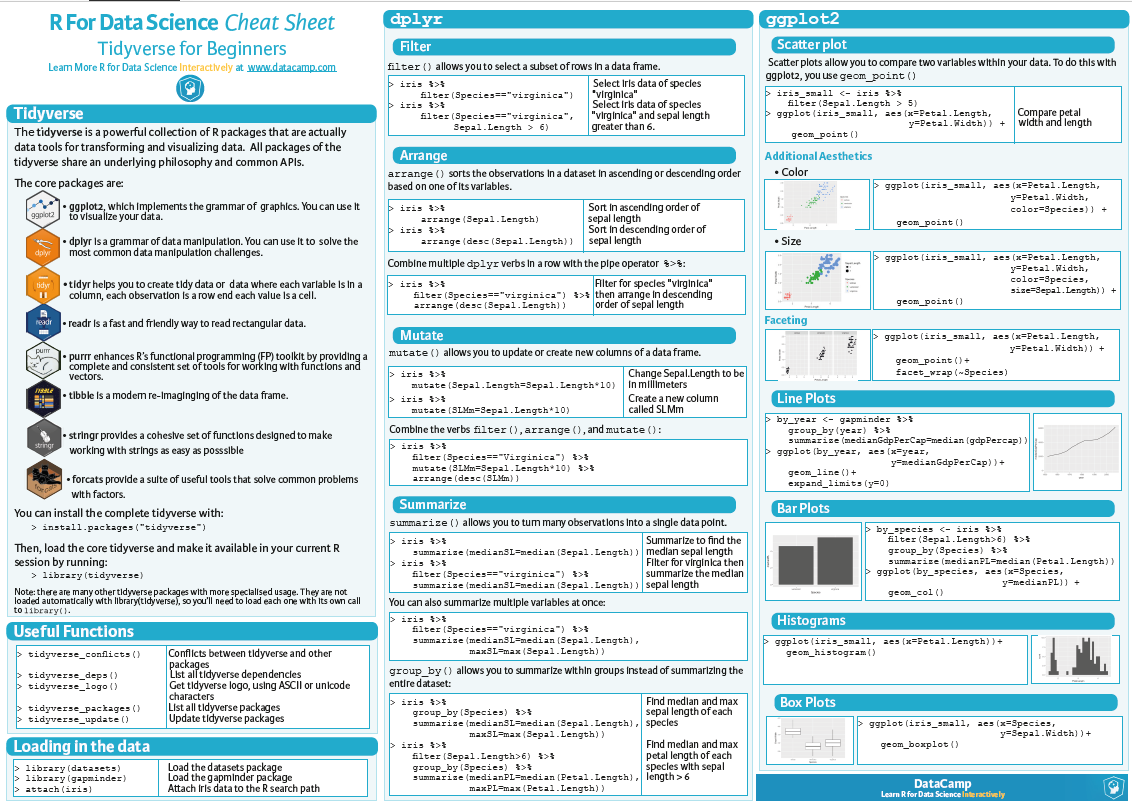
\includegraphics{../external/images/r_cheatsheet_tidy.PNG}

\end{frame}

\hypertarget{part-2-rstudio-project-setup}{%
\section{Part 2: RStudio \& Project
setup}\label{part-2-rstudio-project-setup}}

\begin{frame}{RStudio}
\protect\hypertarget{rstudio}{}

\begin{itemize}
\tightlist
\item
  IDE: Integrated development environment
\item
  RStudio: Does so much

  \begin{itemize}
  \tightlist
  \item
    We scratch the surface here
  \end{itemize}
\item
  Quick walk through

  \begin{itemize}
  \tightlist
  \item
    Followed by specific set up
  \item
    Generally, but
  \item
    Also for this workshop
  \end{itemize}
\end{itemize}

\end{frame}

\begin{frame}{RStudio Setup}
\protect\hypertarget{rstudio-setup}{}

\begin{itemize}
\tightlist
\item
  Download R and Rstudio

  \begin{itemize}
  \tightlist
  \item
    Strongly recommend Microsoft R
    (\url{https://mran.microsoft.com/open})
  \item
    Comes with Intel MKL
  \end{itemize}
\item
  Plain R is fine (\url{https://cran.r-project.org/})

  \begin{itemize}
  \tightlist
  \item
    Can relink to faster libraries
  \end{itemize}
\item
  Download RStudio (\url{https://www.rstudio.com/})
\end{itemize}

\end{frame}

\begin{frame}{RStudio Environment}
\protect\hypertarget{rstudio-environment}{}

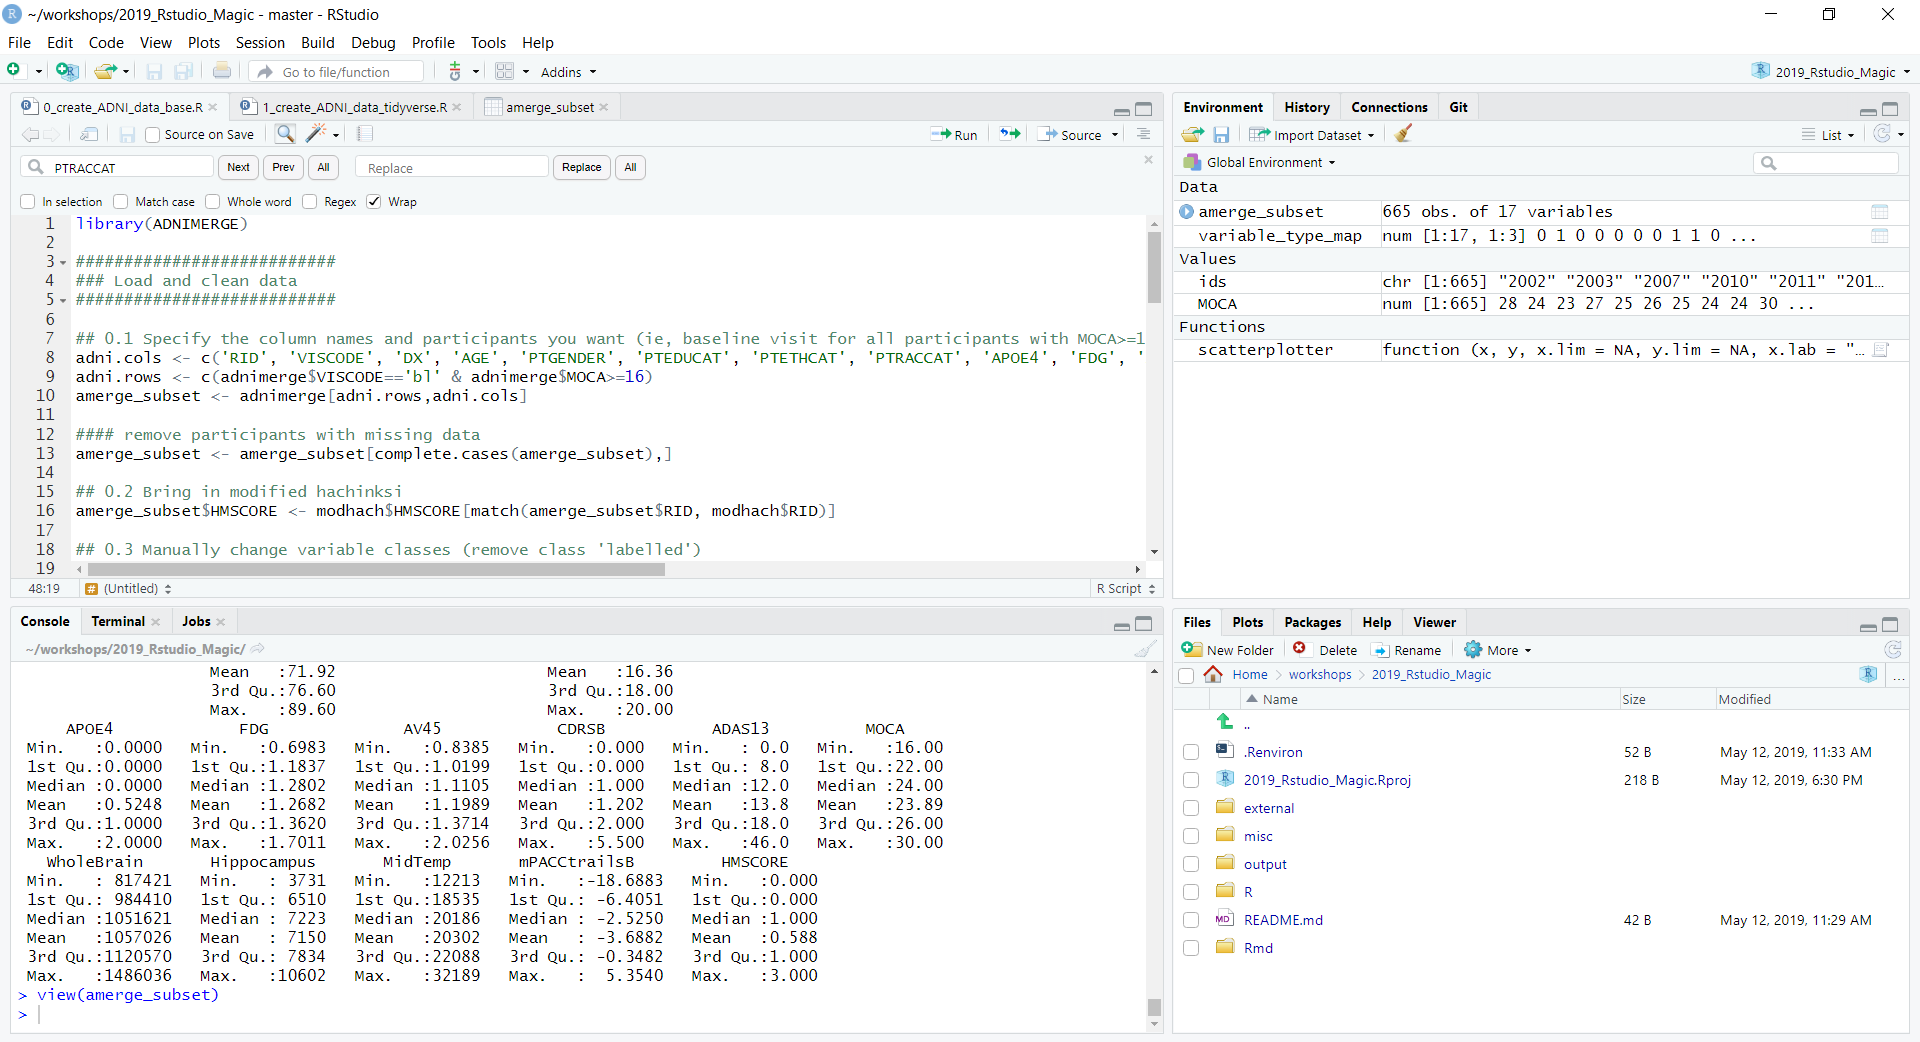
\includegraphics{../external/images/rstudio_terminal_0.PNG}

\end{frame}

\begin{frame}{RStudio Environment}
\protect\hypertarget{rstudio-environment-1}{}

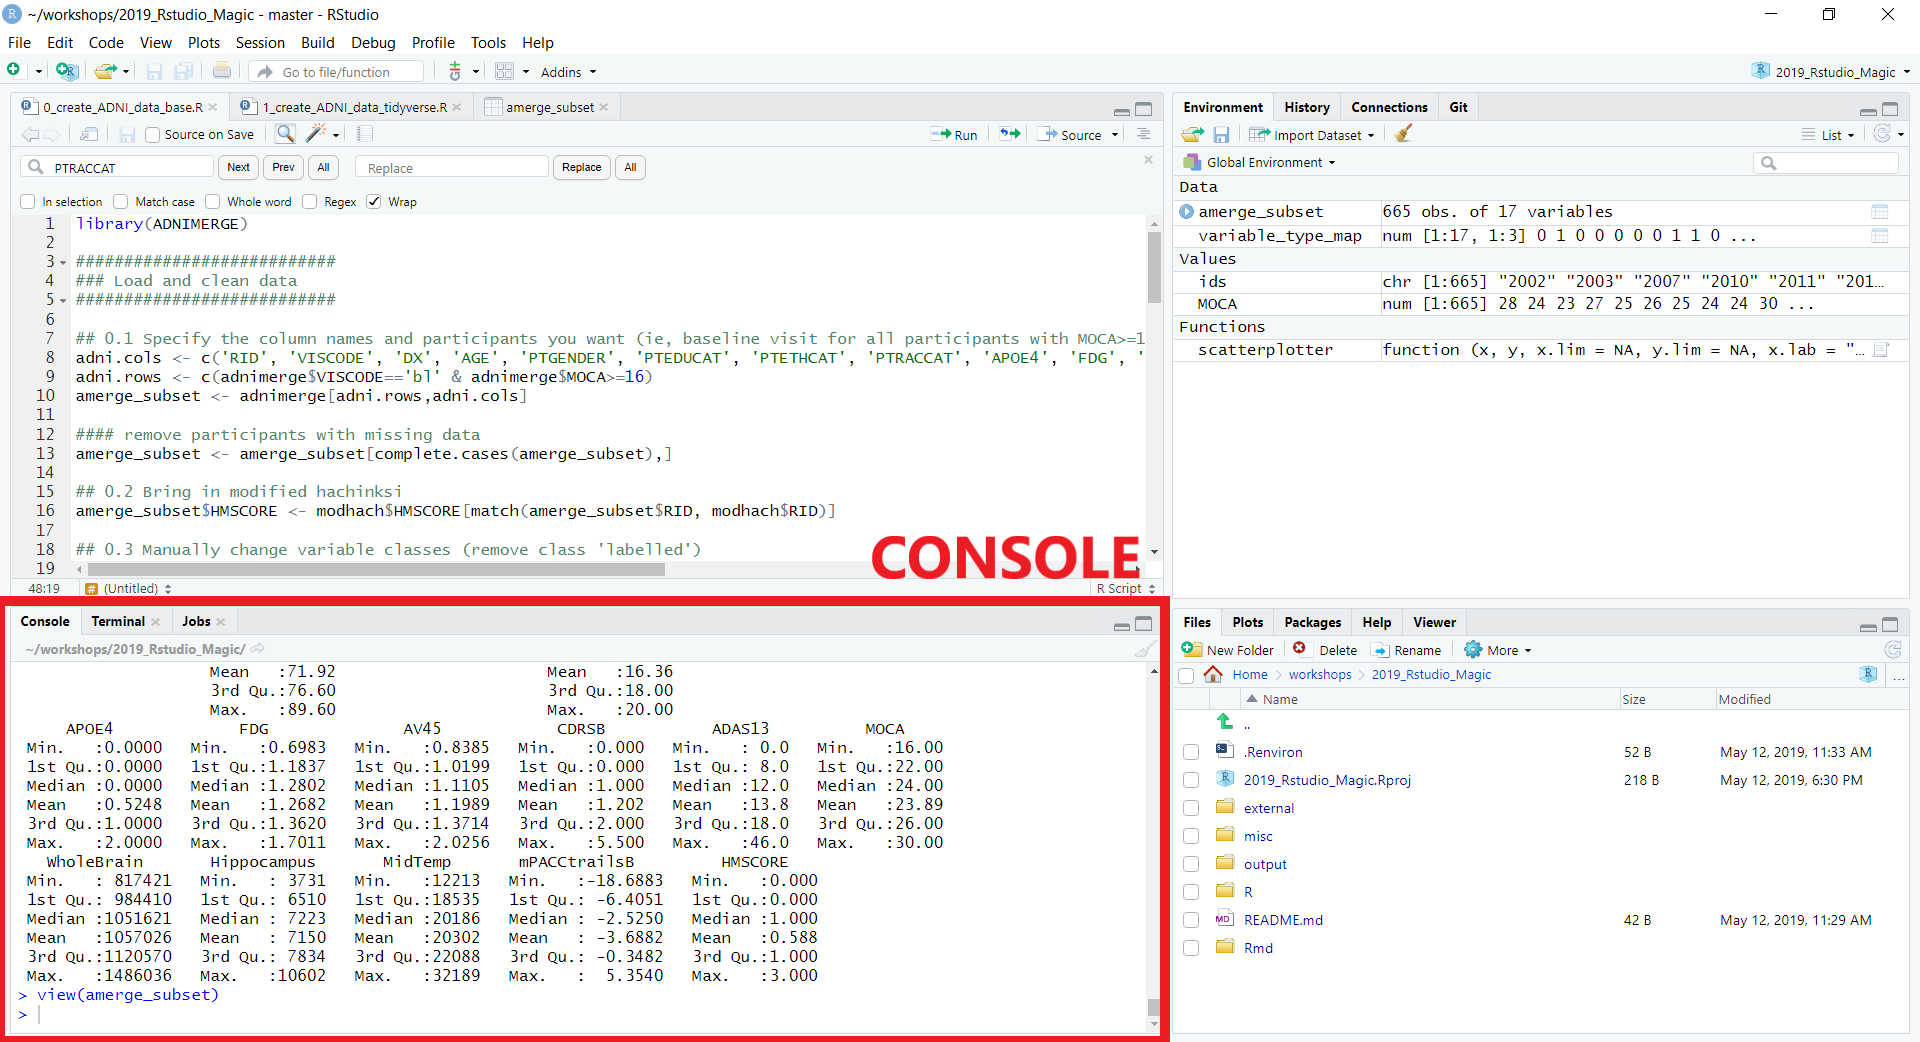
\includegraphics{../external/images/rstudio_terminal_1_CONSOLE.png}

\end{frame}

\begin{frame}{RStudio Environment}
\protect\hypertarget{rstudio-environment-2}{}

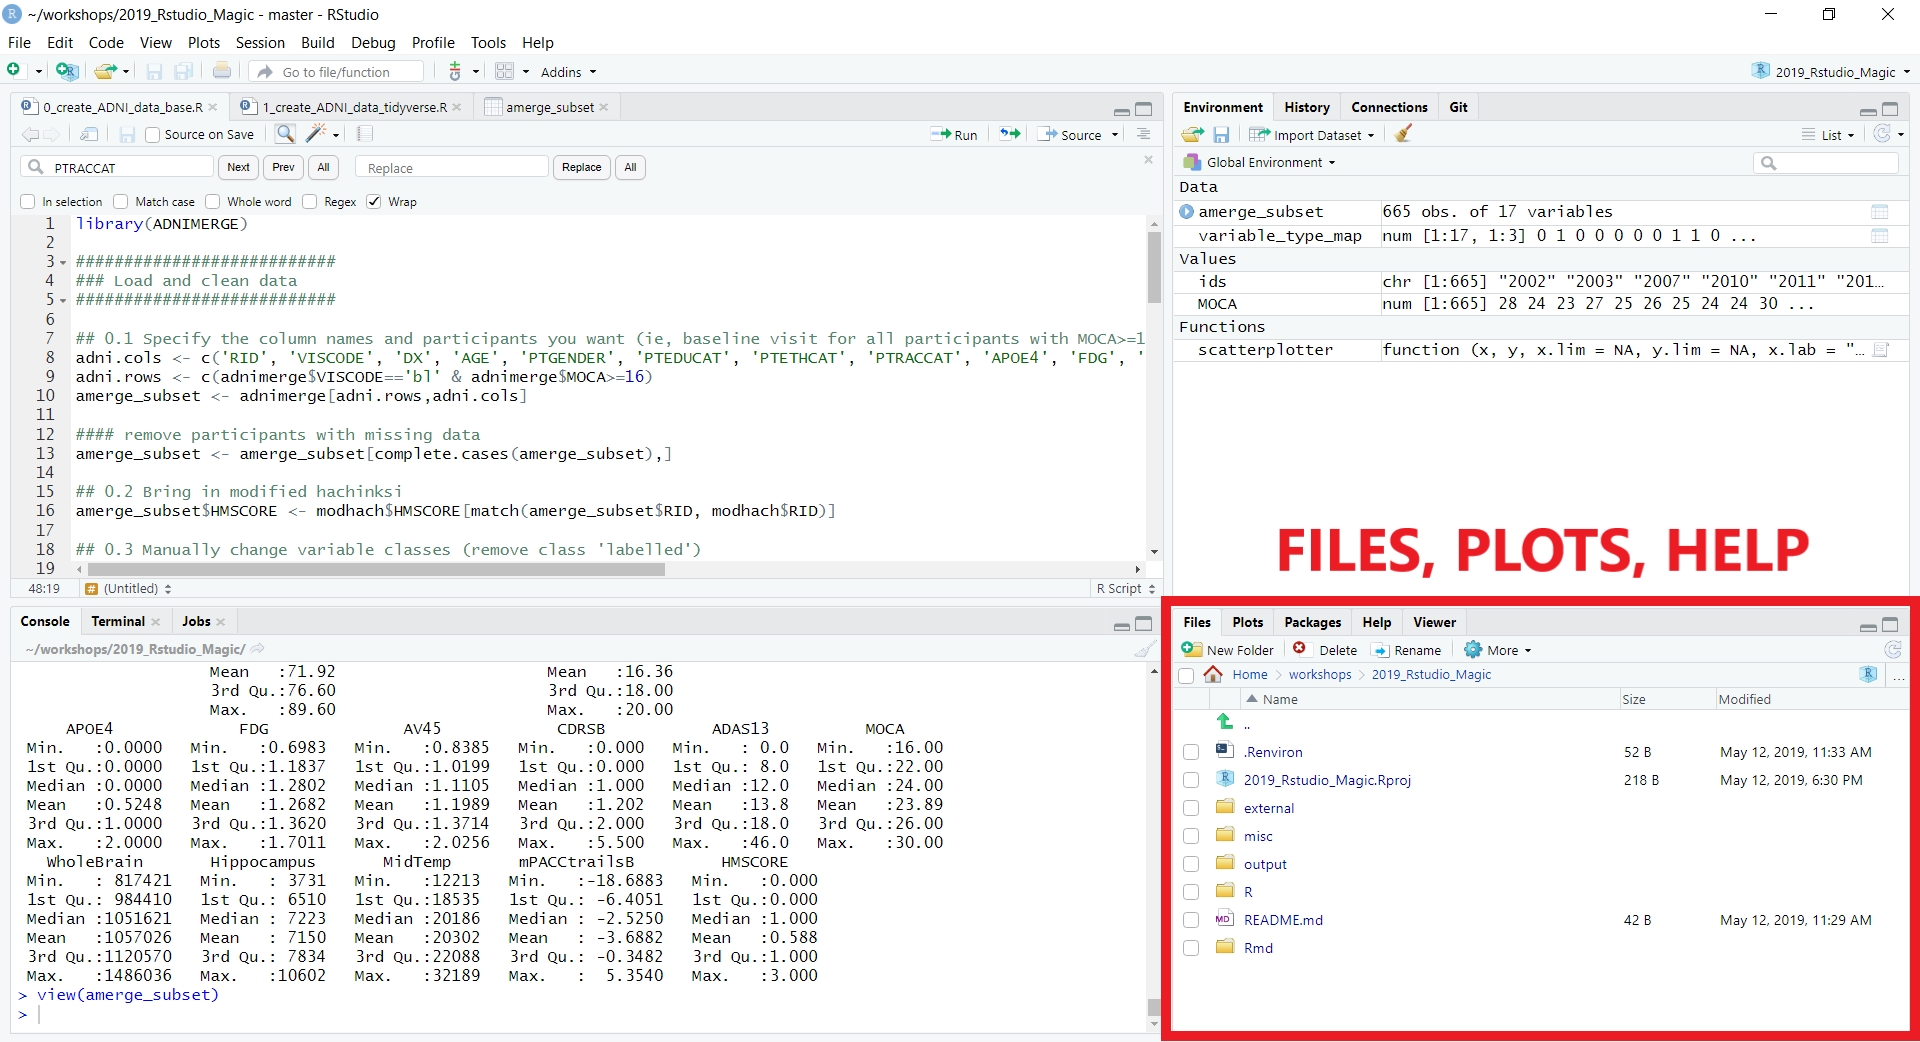
\includegraphics{../external/images/rstudio_terminal_2_FILES.png}

\end{frame}

\begin{frame}{RStudio Environment}
\protect\hypertarget{rstudio-environment-3}{}

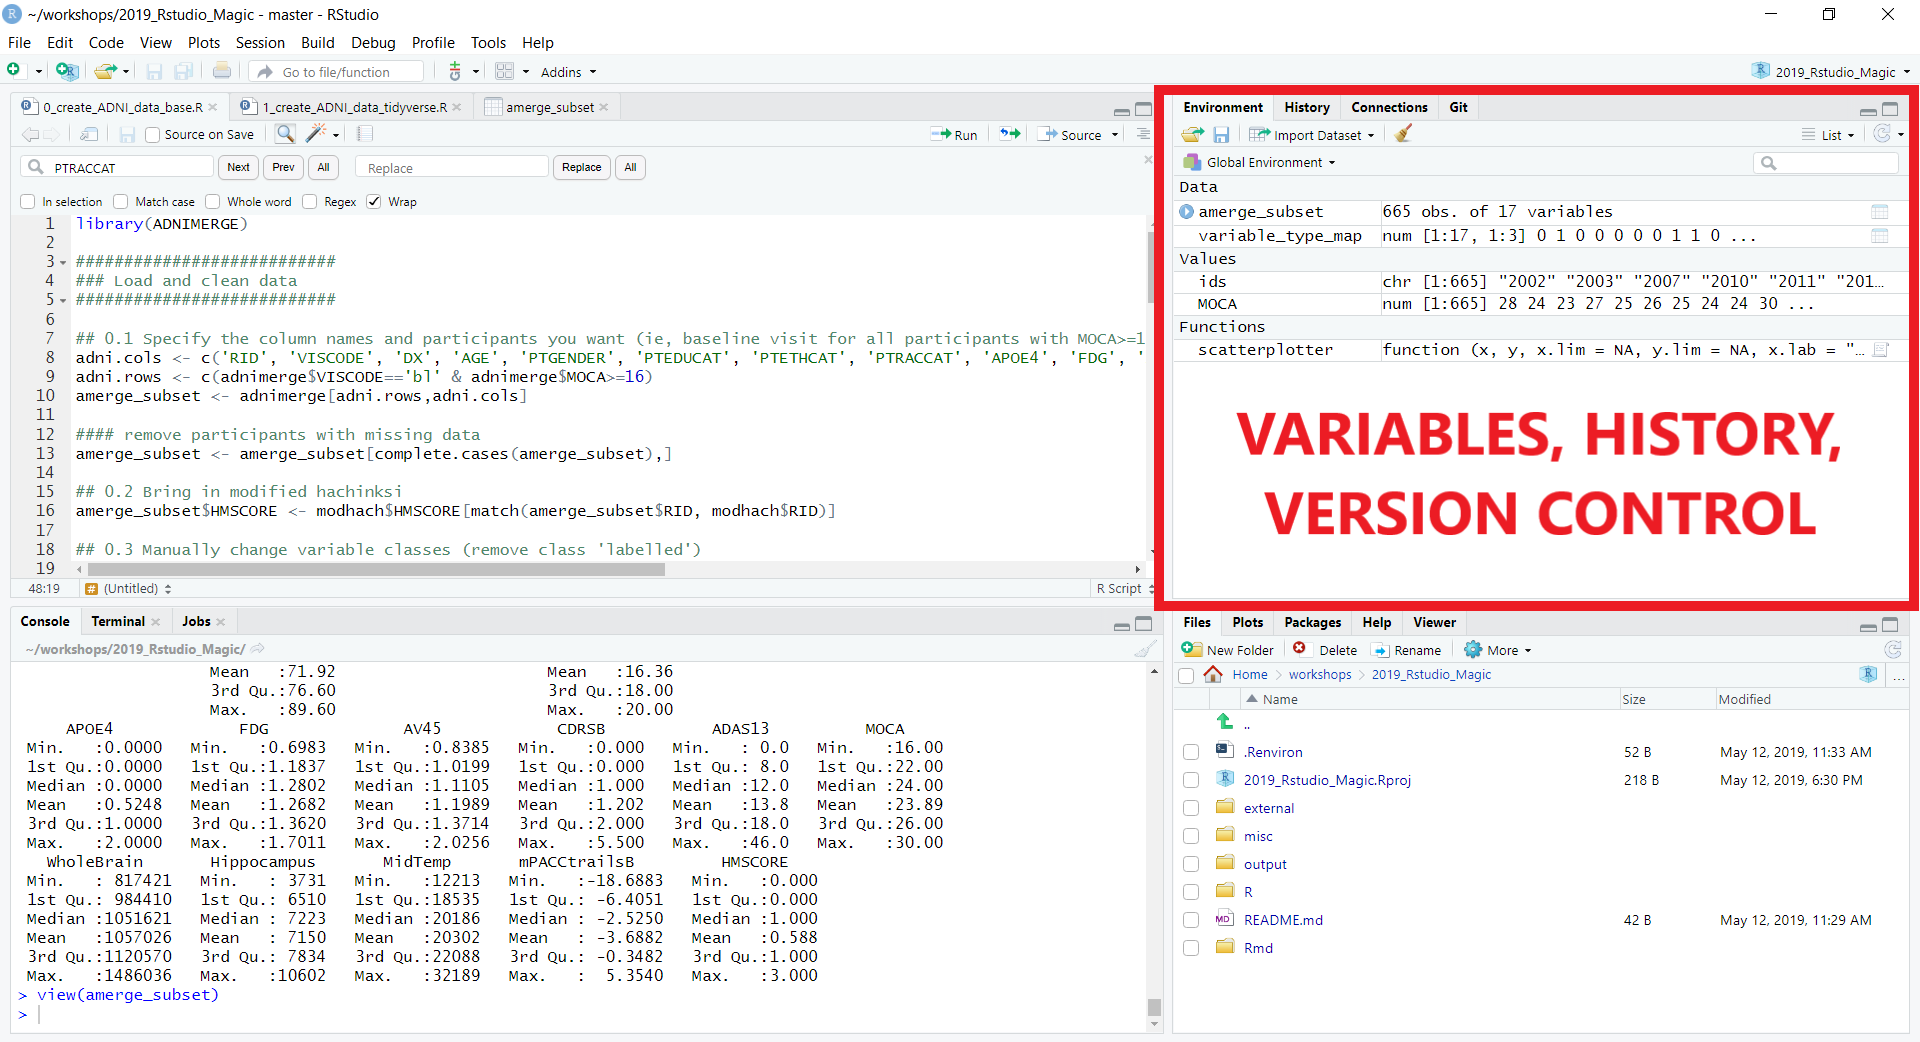
\includegraphics{../external/images/rstudio_terminal_3_ENV.png}

\end{frame}

\begin{frame}{RStudio Environment}
\protect\hypertarget{rstudio-environment-4}{}

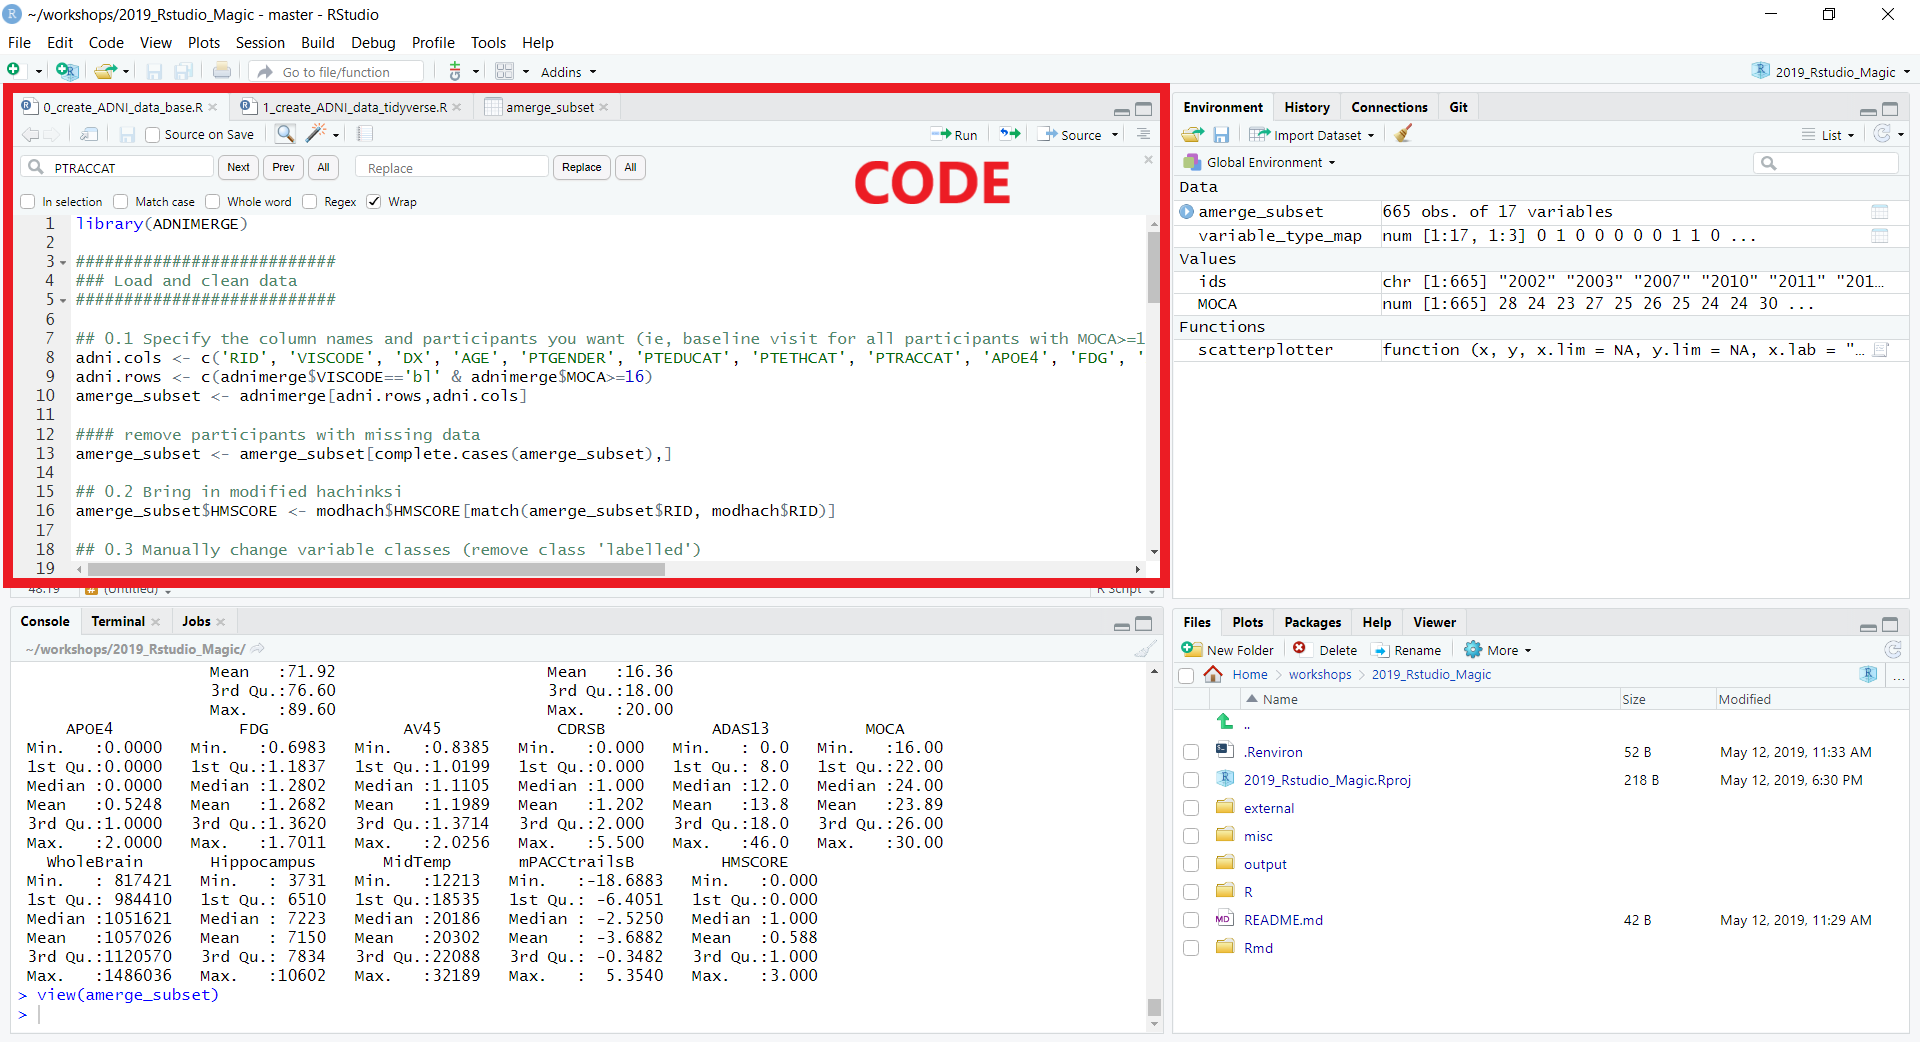
\includegraphics{../external/images/rstudio_terminal_4_CODE.png}

\end{frame}

\begin{frame}{RStudio Environment}
\protect\hypertarget{rstudio-environment-5}{}

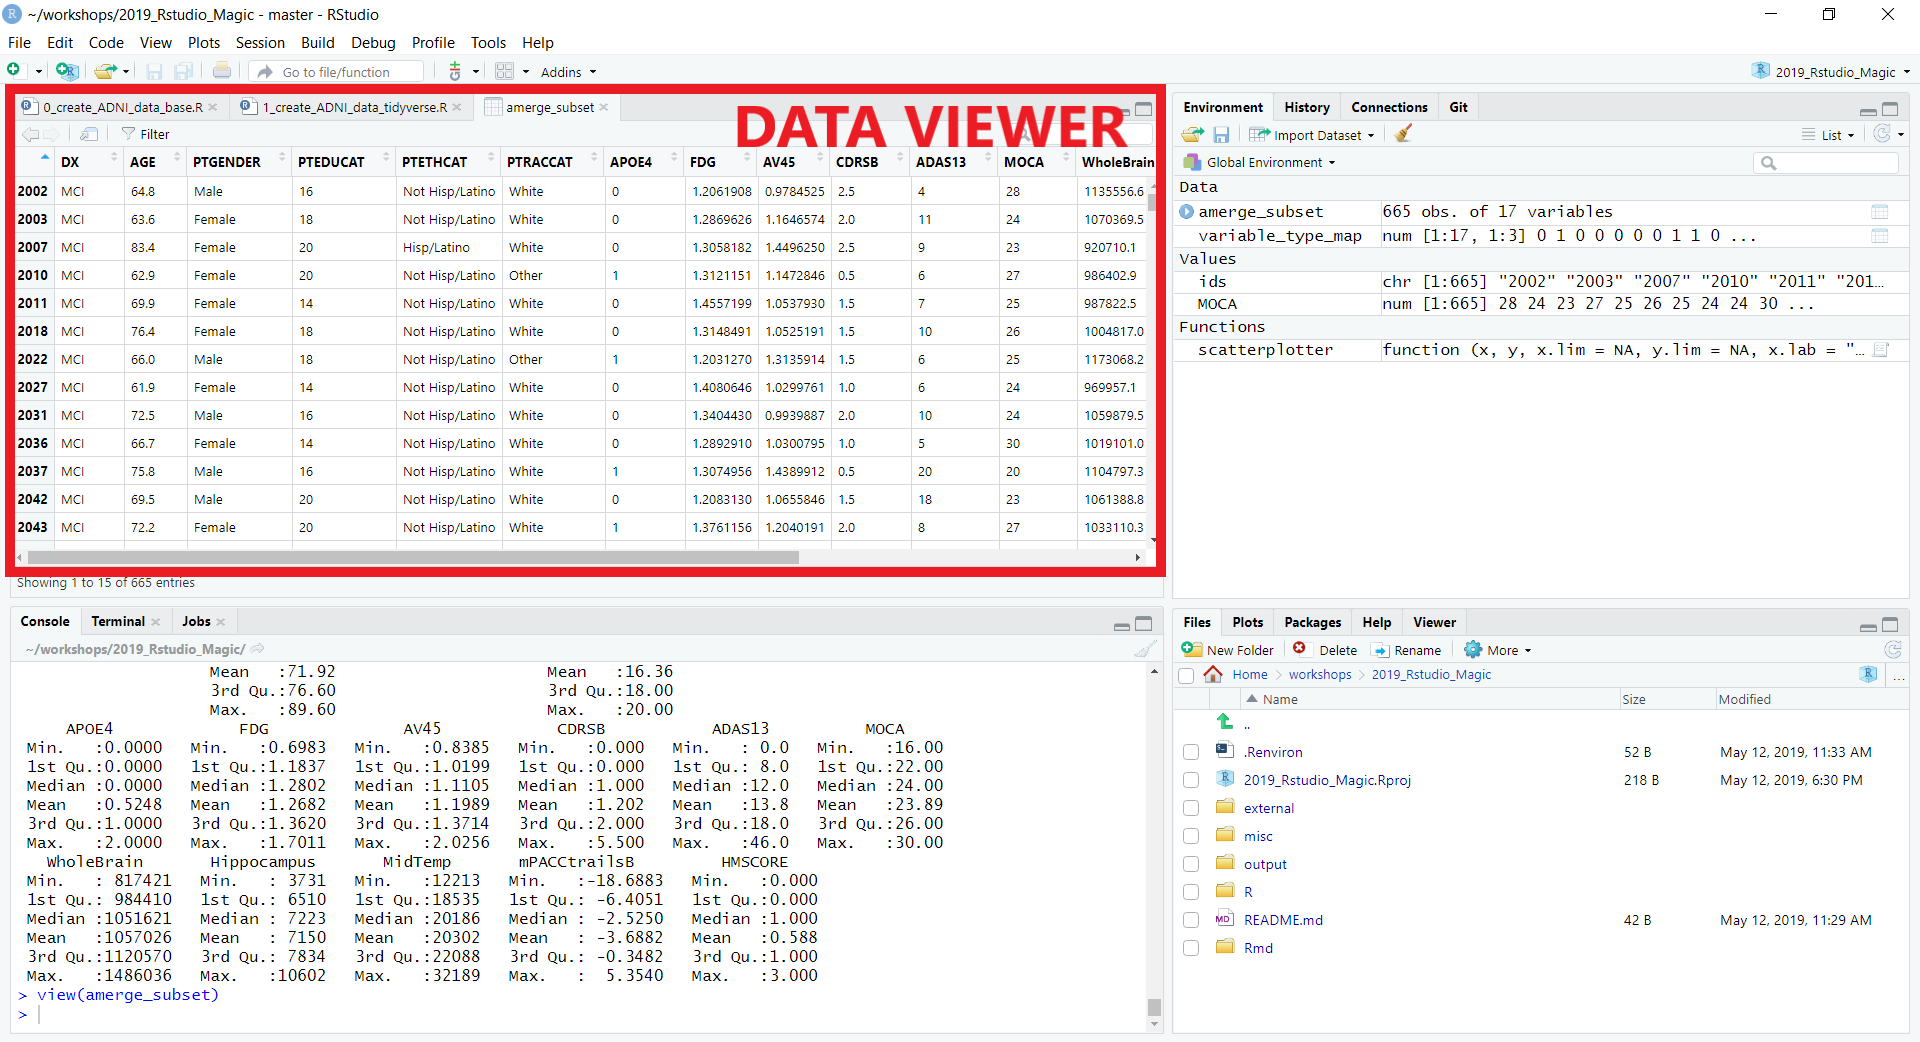
\includegraphics{../external/images/rstudio_terminal_5_DATA.png}

\end{frame}

\begin{frame}{Some benefits of RStudio}
\protect\hypertarget{some-benefits-of-rstudio}{}

\begin{itemize}
\tightlist
\item
  Built-in integration with version control (git or SVN)
\item
  R Markdown

  \begin{itemize}
  \tightlist
  \item
    Save and execute code
  \item
    Generate high quality reports that can be shared
  \item
    Create presentations (like this one!)
  \item
    Even write papers
  \item
    This workshop

    \begin{itemize}
    \tightlist
    \item
      See
      \url{https://github.com/jennyrieck/workshops/tree/master/2019_Rstudio_Magic}
    \end{itemize}
  \end{itemize}
\item
  Python, D3 (JavaScript), SQL, Shiny, LaTeX, Git/SVN, HTML/CSS, and so
  much more.
\end{itemize}

\end{frame}

\begin{frame}{RStudio is more}
\protect\hypertarget{rstudio-is-more}{}

\begin{itemize}
\tightlist
\item
  Not just an IDE
\item
  A company
\item
  A community
\item
  A conference
\item
  A centralized resource
\end{itemize}

\end{frame}

\begin{frame}{RStudio Resources}
\protect\hypertarget{rstudio-resources}{}

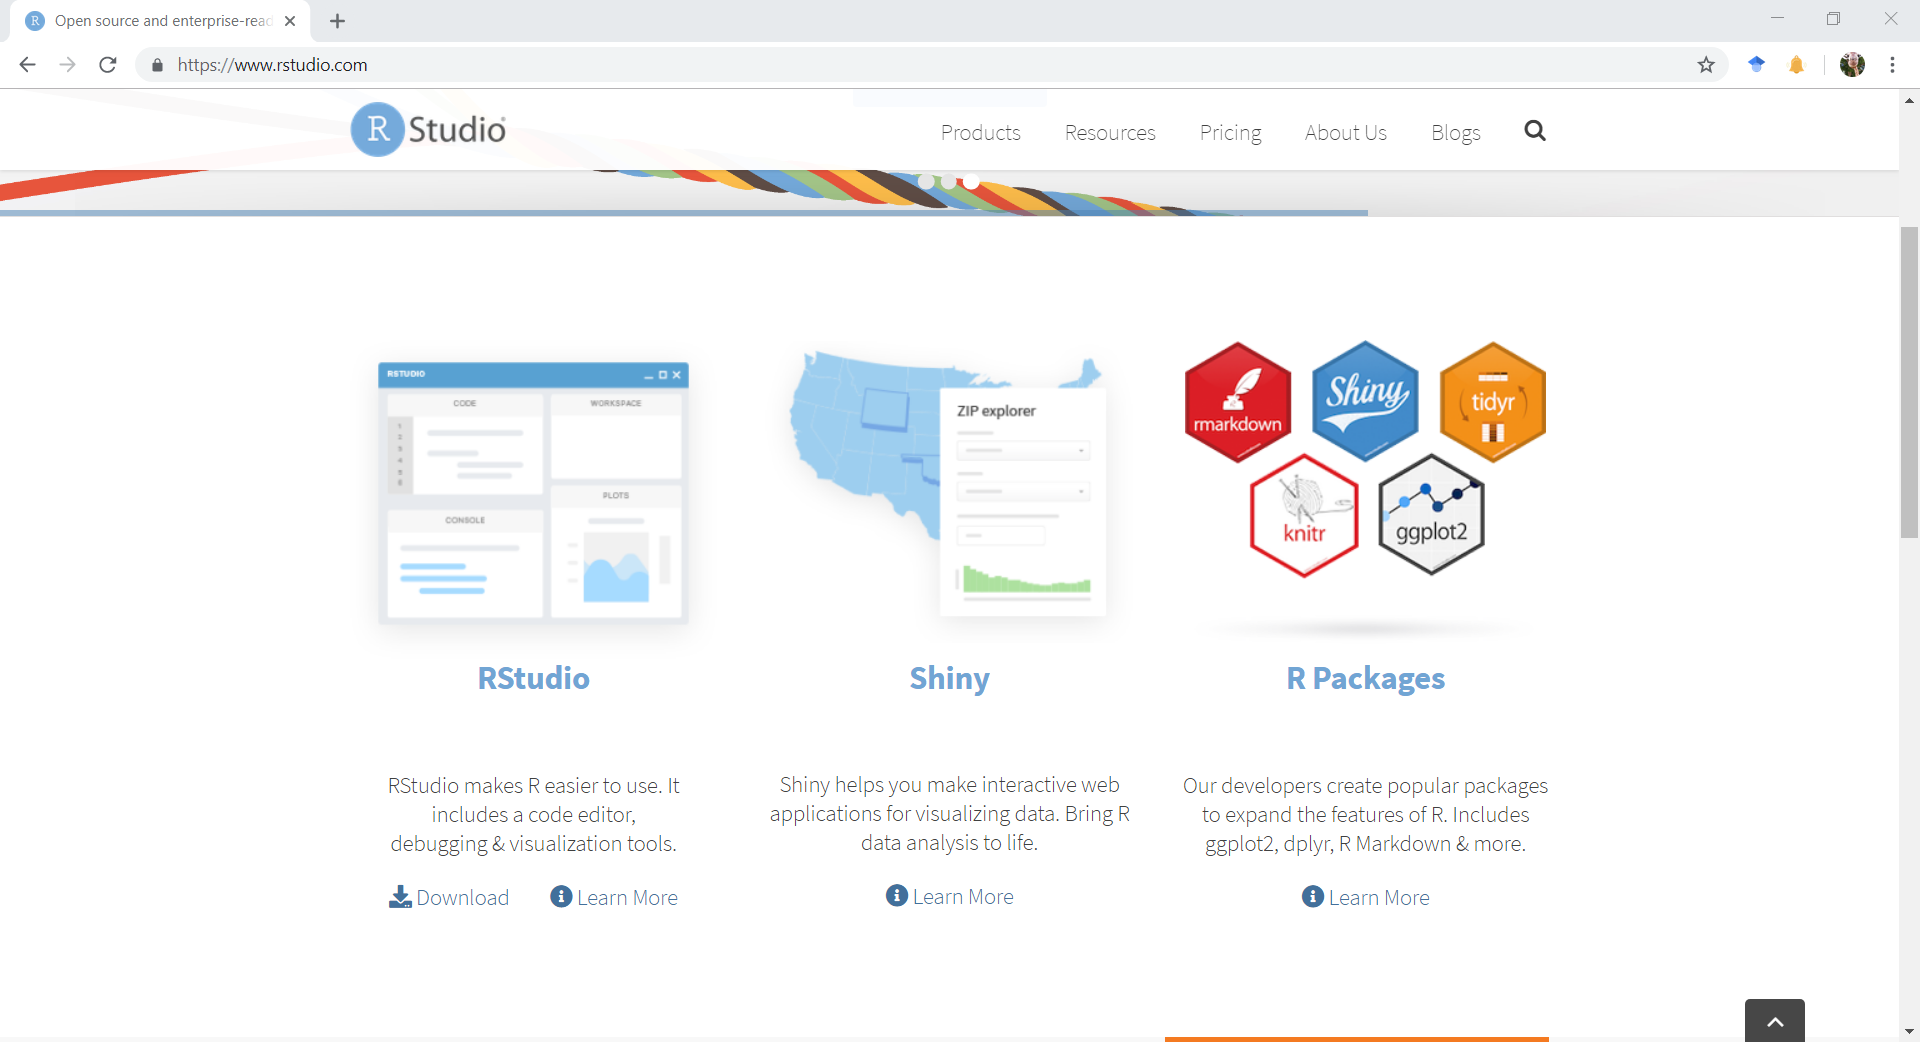
\includegraphics{../external/images/rstudio_dot_com_1_main.PNG}

\end{frame}

\begin{frame}{RStudio Resources}
\protect\hypertarget{rstudio-resources-1}{}

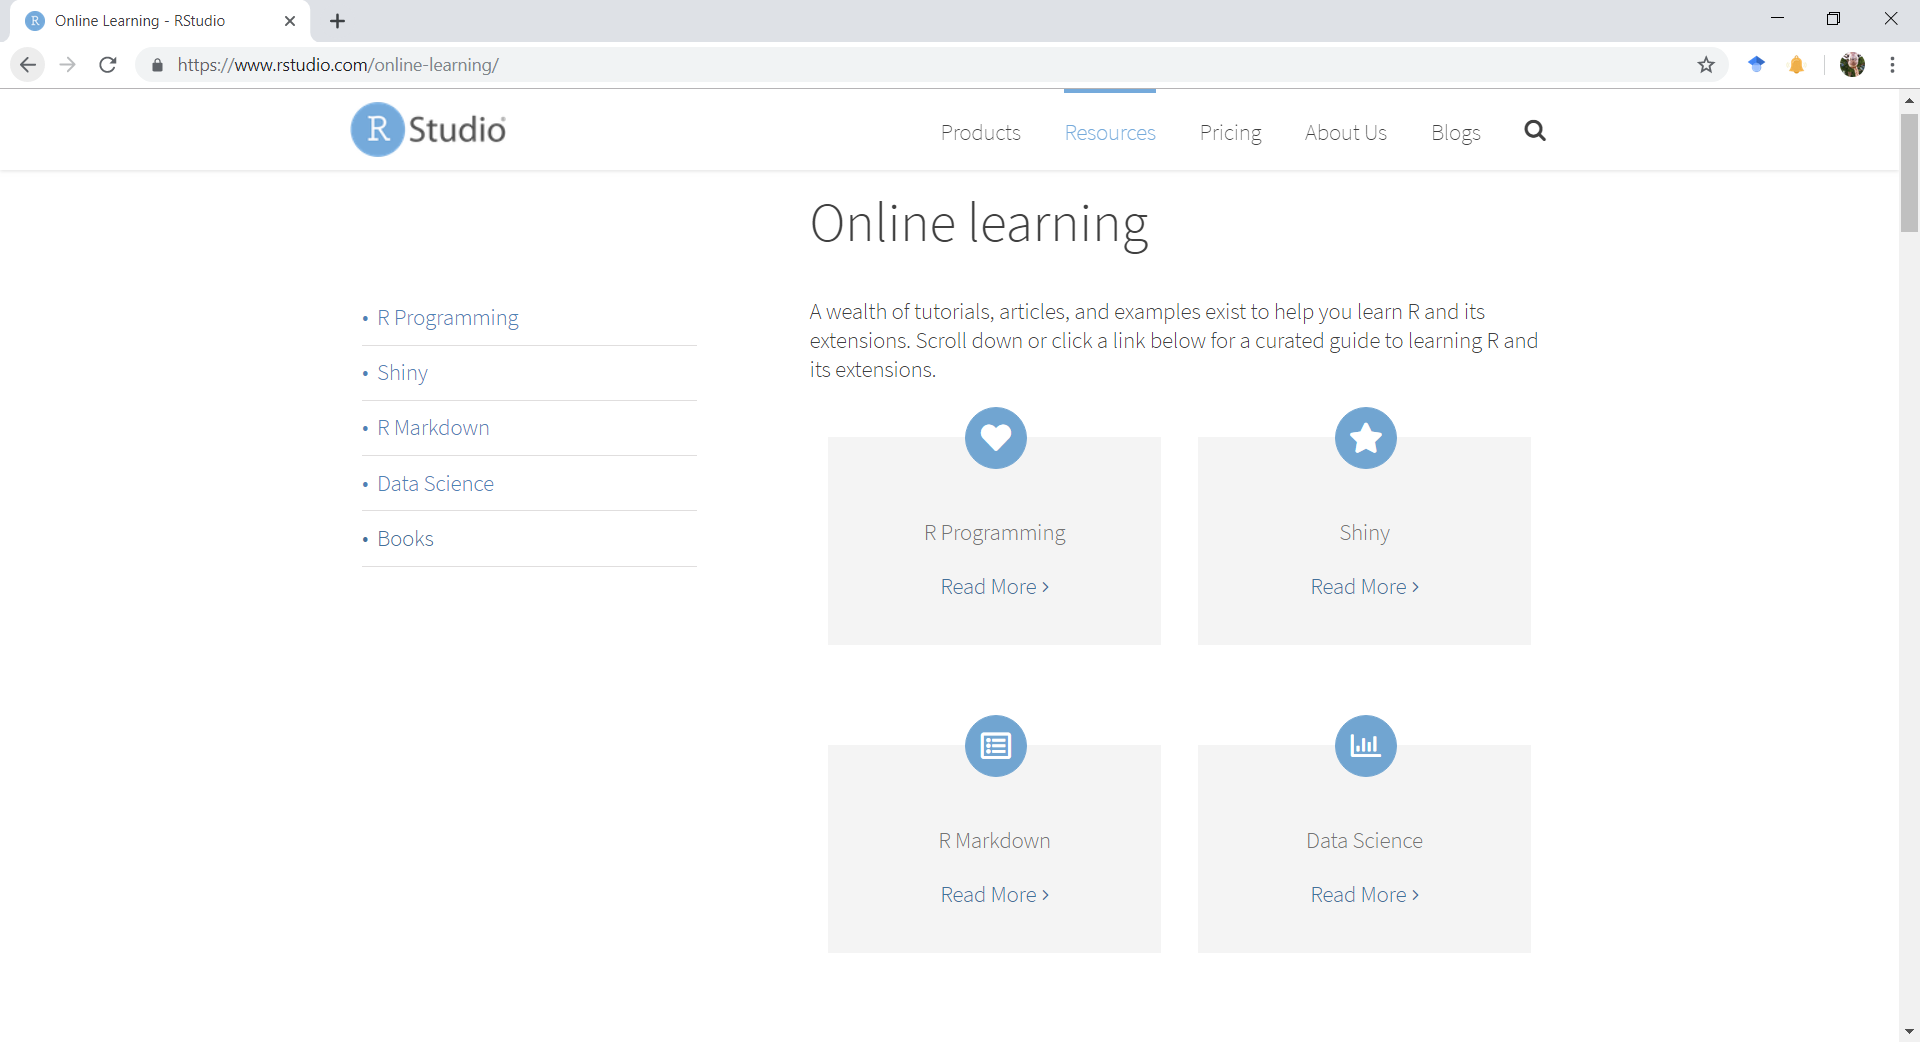
\includegraphics{../external/images/rstudio_dot_com_2_learning.PNG}

\end{frame}

\begin{frame}{RStudio Resources}
\protect\hypertarget{rstudio-resources-2}{}

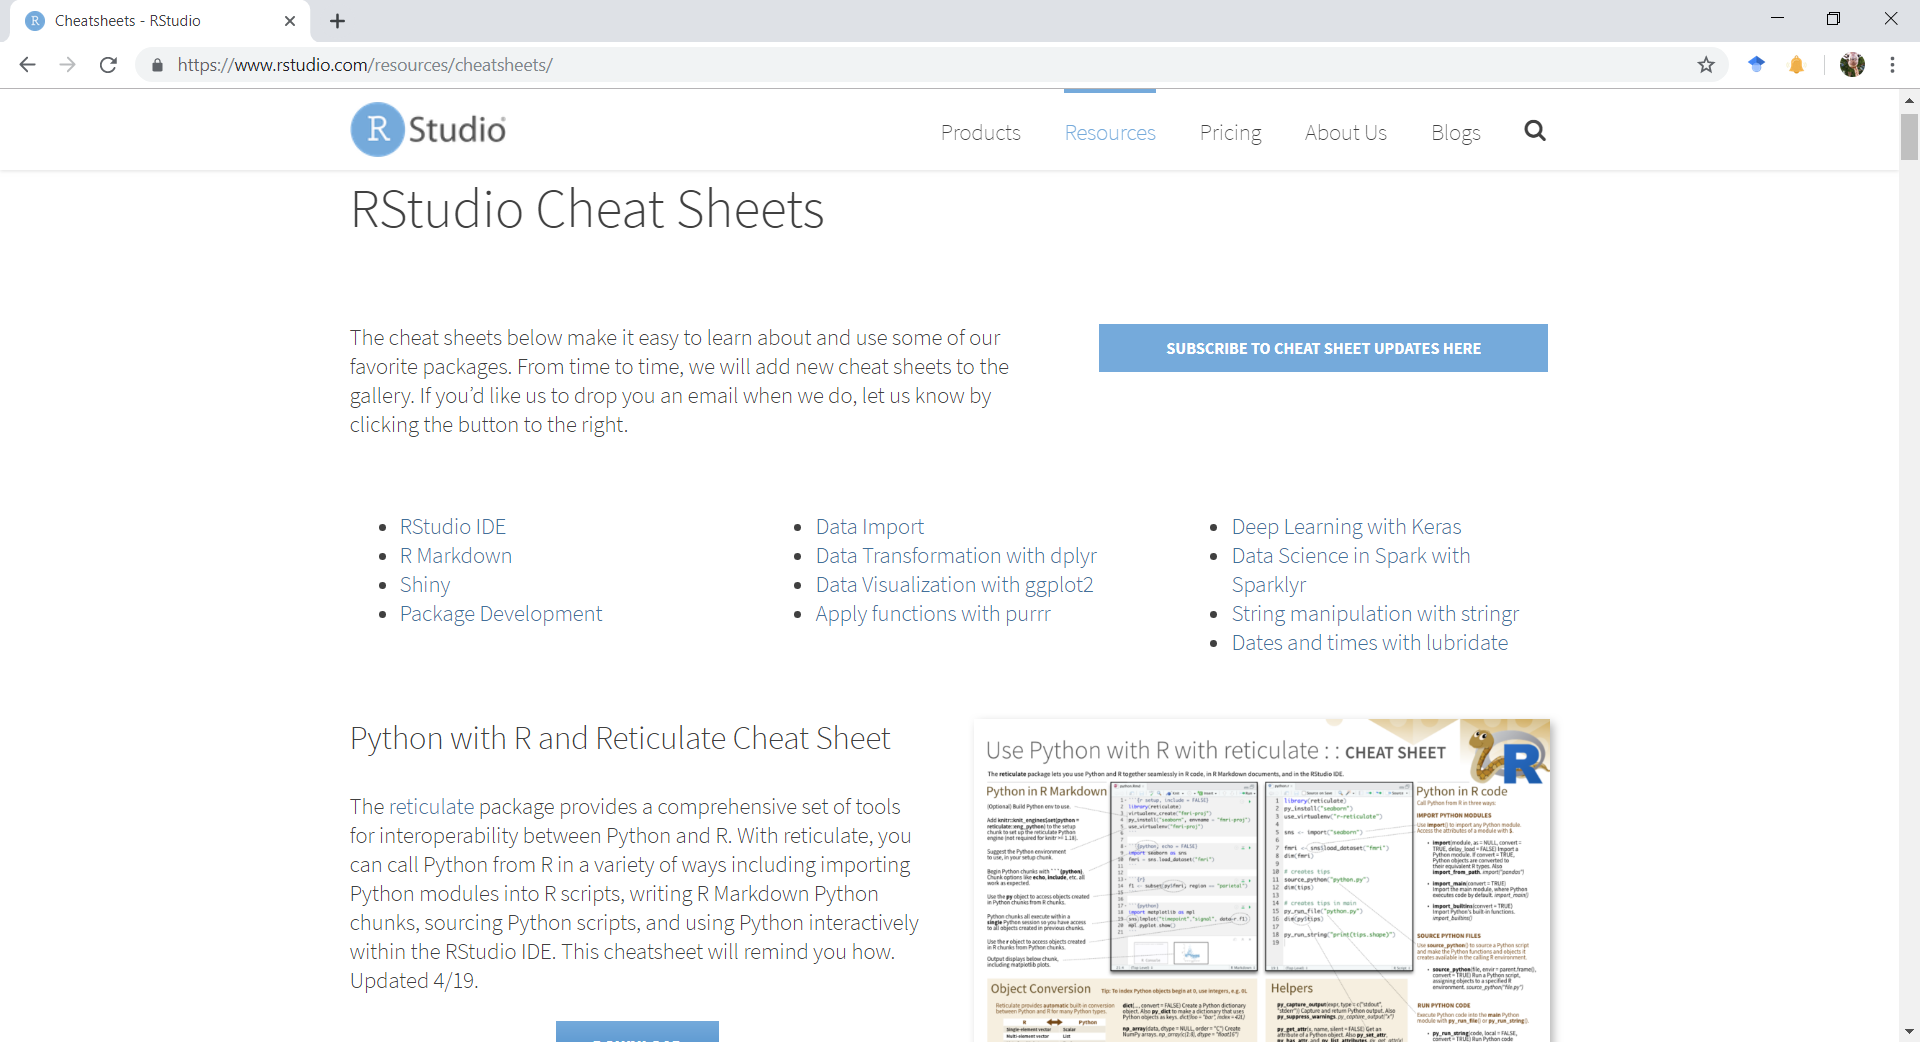
\includegraphics{../external/images/rstudio_dot_com_3_cheats.PNG}

\end{frame}

\begin{frame}{Project and Environment Setup}
\protect\hypertarget{project-and-environment-setup}{}

\begin{itemize}
\tightlist
\item
  Special \& hidden files
\item
  Having a structure
\end{itemize}

\end{frame}

\begin{frame}{RStudio Setup}
\protect\hypertarget{rstudio-setup-1}{}

\begin{itemize}
\tightlist
\item
  See \url{https://jennybc.github.io/2014-05-12-ubc/r-setup.html} for a
  detailed guide
\end{itemize}

\end{frame}

\begin{frame}{For safety \& collaboration}
\protect\hypertarget{for-safety-collaboration}{}

\begin{itemize}
\tightlist
\item
  RStudio projects

  \begin{itemize}
  \tightlist
  \item
    ``RStudio projects make it straightforward to divide your work into
    multiple contexts, each with their own working directory, workspace,
    history, and source documents.''
  \item
    Allows for return to key states
  \end{itemize}
\item
  .Rproj files

  \begin{itemize}
  \tightlist
  \item
    Basically a text file with some parameters for start up
    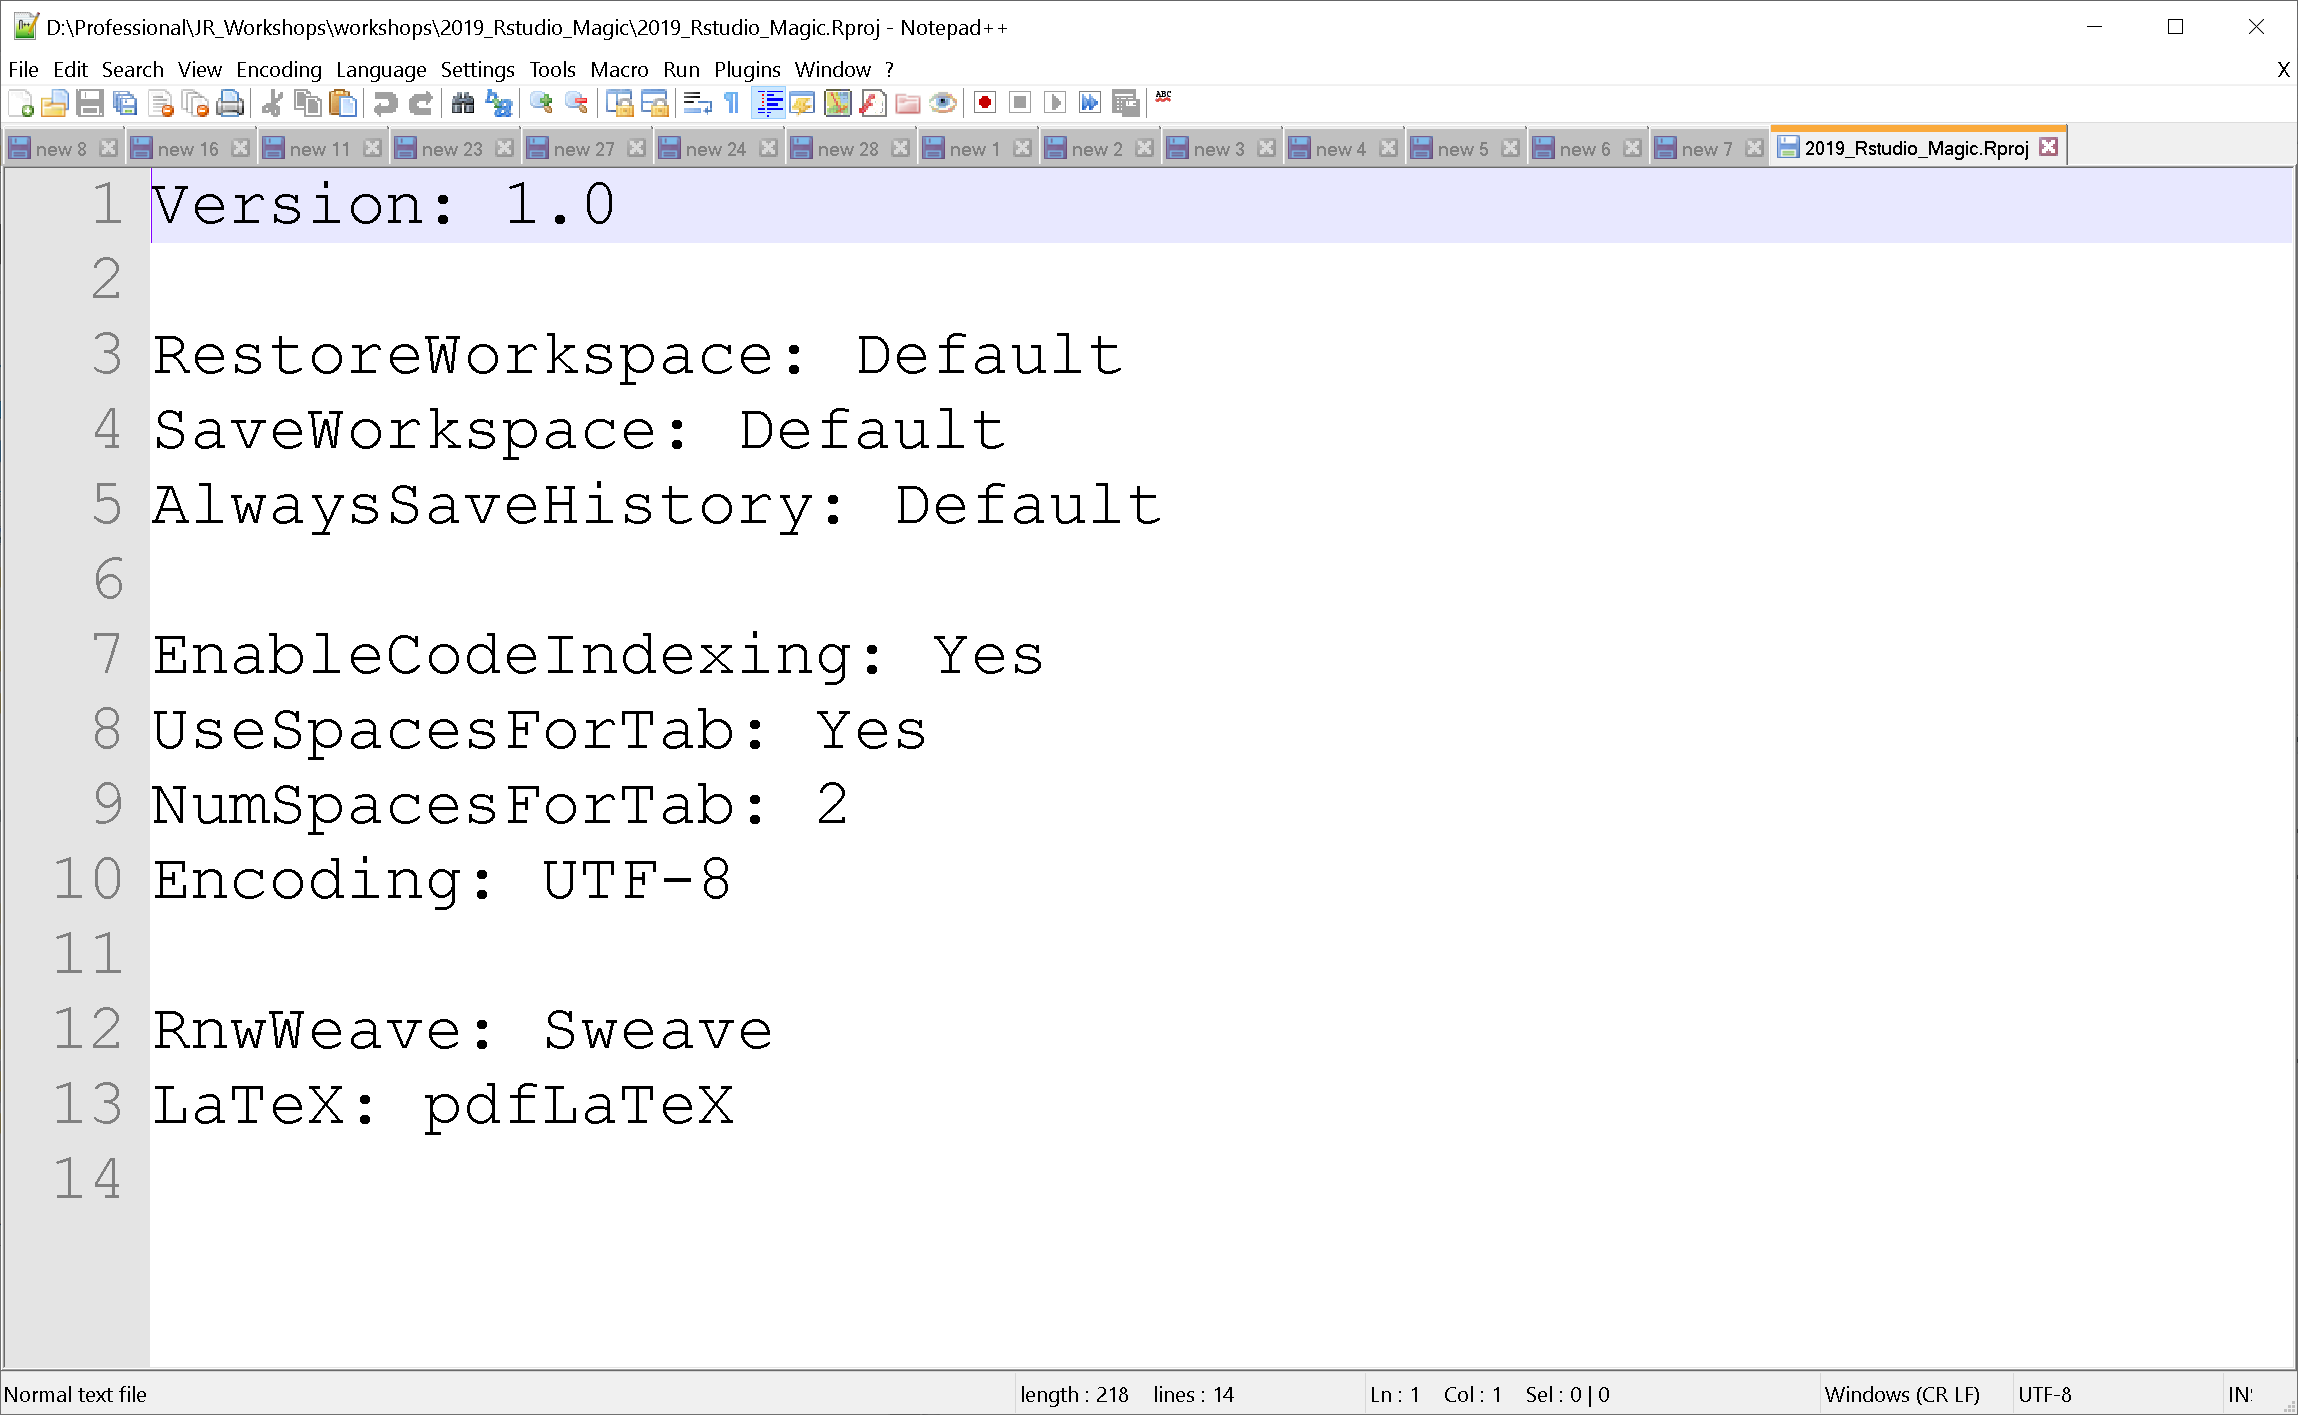
\includegraphics[width=0.5\textwidth,height=\textheight]{../external/images/Rproj_inside.PNG}
  \end{itemize}
\end{itemize}

\end{frame}

\begin{frame}{Projects}
\protect\hypertarget{projects}{}

Create a new one for:

\begin{itemize}
\tightlist
\item
  a folder
\item
  packages
\item
  (and from) git repos:
  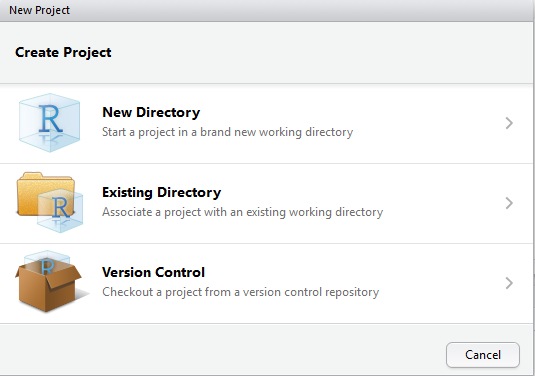
\includegraphics[width=0.75\textwidth,height=\textheight]{../external/images/setup_2_rstudio_project.PNG}
\end{itemize}

\end{frame}

\begin{frame}{Git \& Projects}
\protect\hypertarget{git-projects}{}

\begin{itemize}
\tightlist
\item
  Git
\item
  Download git and link executable within RStudio
  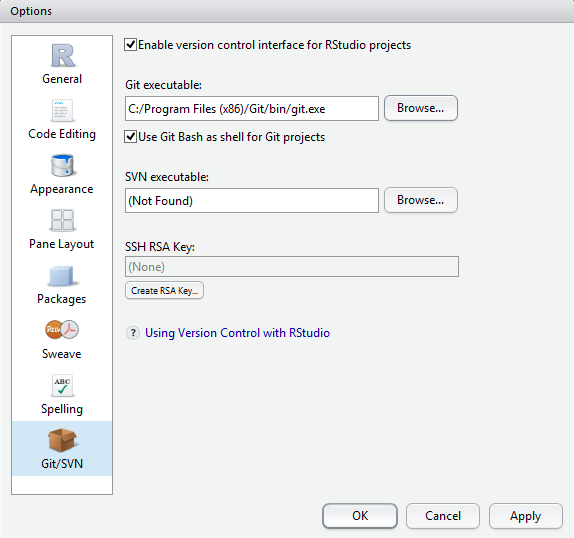
\includegraphics[width=0.6\textwidth,height=\textheight]{../external/images/setup_1_rstudio_git.PNG}
\end{itemize}

\end{frame}

\begin{frame}[fragile]{Format .gitignore}
\protect\hypertarget{format-.gitignore}{}

\begin{itemize}
\tightlist
\item
  File types to ignore via version control
\item
  \texttt{**} before each extentions will match directories anywhere in
  the repo
\end{itemize}

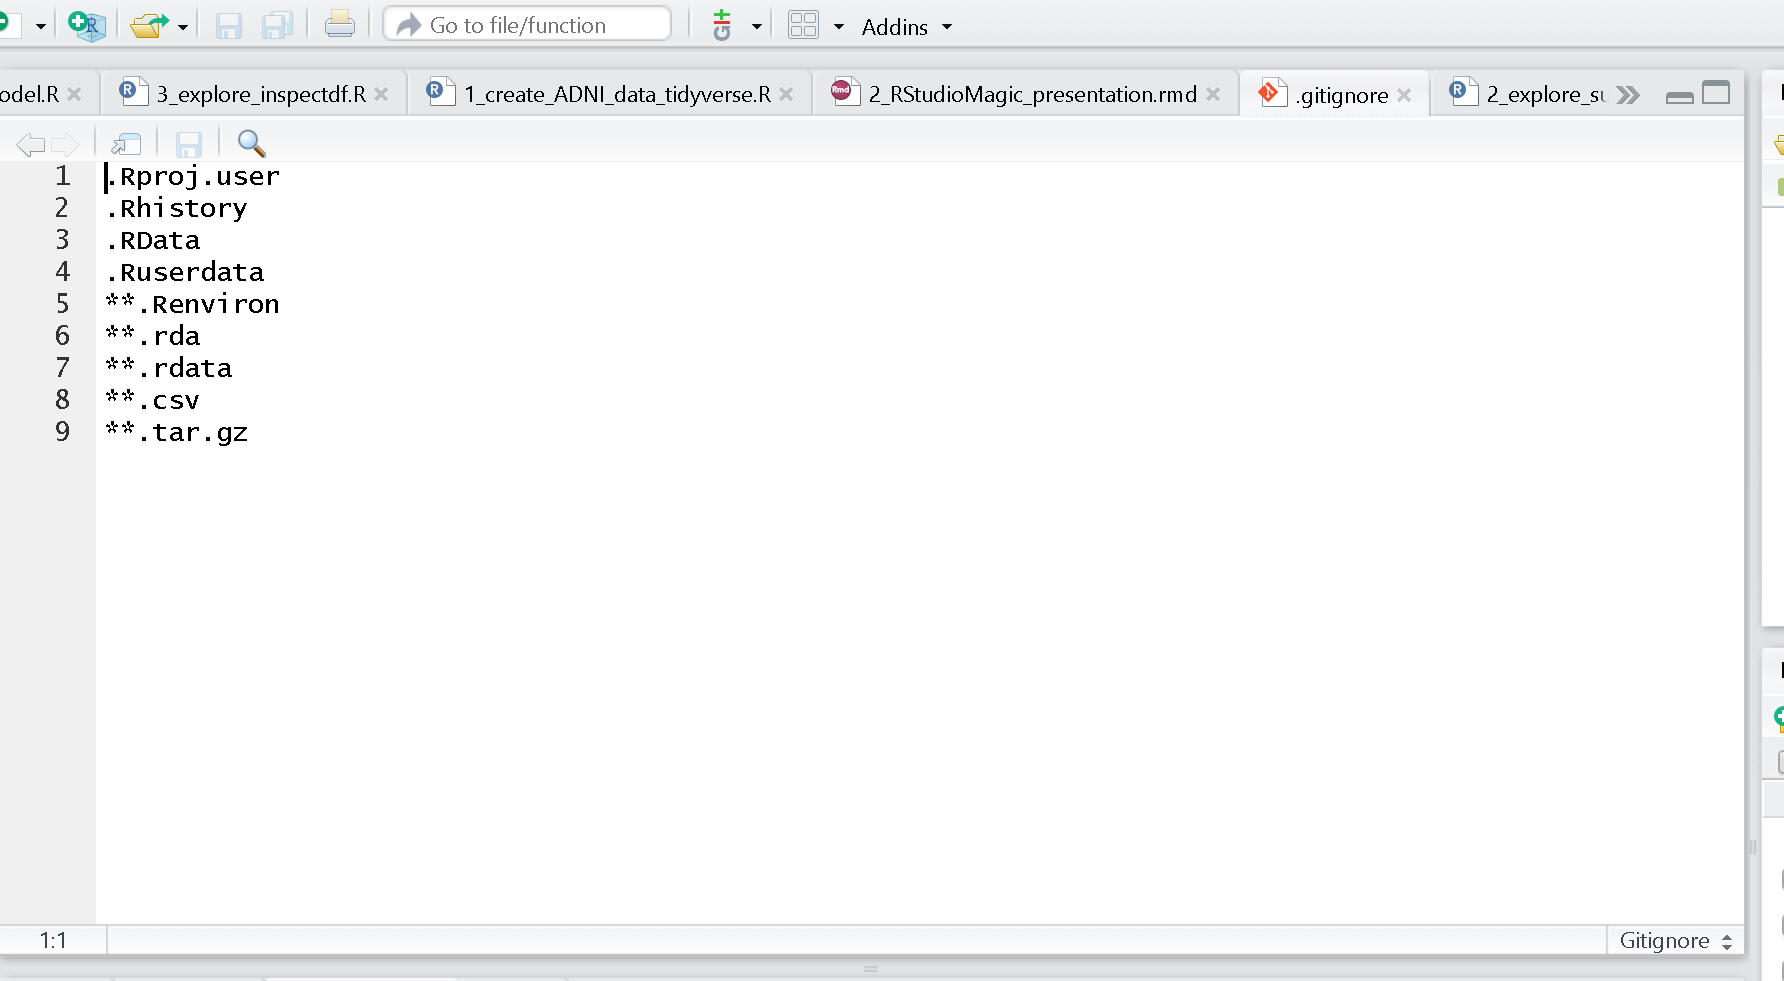
\includegraphics[width=0.75\textwidth,height=\textheight]{../external/images/gitignore.PNG}

\end{frame}

\begin{frame}{Environmental variables}
\protect\hypertarget{environmental-variables}{}

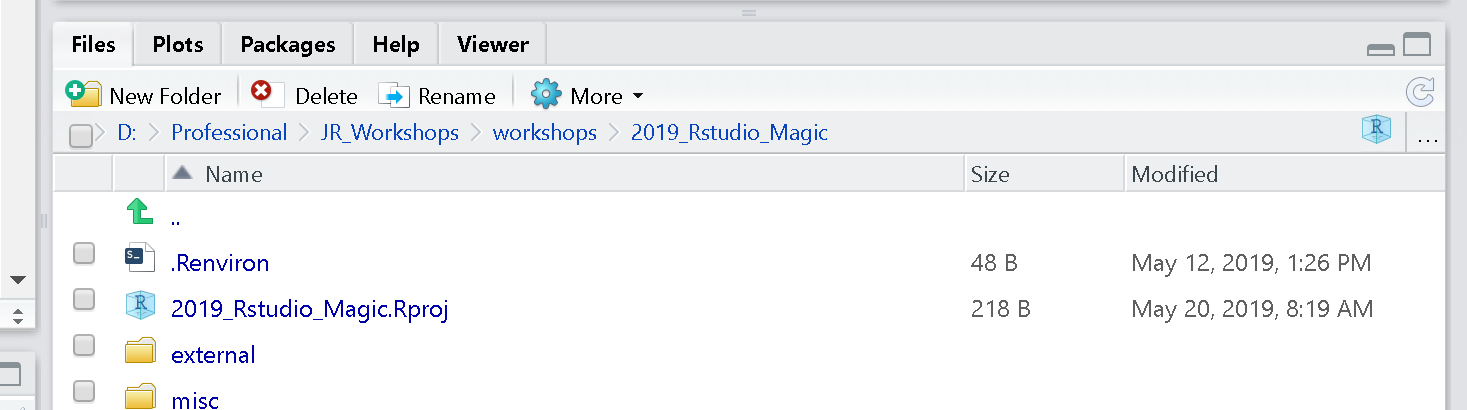
\includegraphics[width=0.6\textwidth,height=\textheight]{../external/images/Revniron.PNG}

\end{frame}

\begin{frame}[fragile]{Format environmental variables}
\protect\hypertarget{format-environmental-variables}{}

\begin{itemize}
\tightlist
\item
  Set environmental variables (ie, directory location of data) to make
  code generalizable across computers

  \begin{itemize}
  \tightlist
  \item
    Don't commit or share these
  \end{itemize}
\item
  In \textbf{your} project folder create a \texttt{.Renviron} file and
  define variables

  \begin{itemize}
  \tightlist
  \item
    Jenny's:
  \end{itemize}

  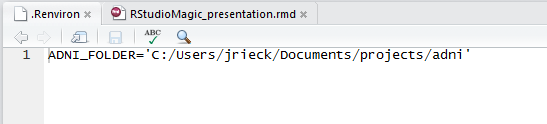
\includegraphics[width=0.6\textwidth,height=\textheight]{../external/images/setup_3_rstudio_project_environ.PNG}

  \begin{itemize}
  \tightlist
  \item
    Derek's:
  \end{itemize}

  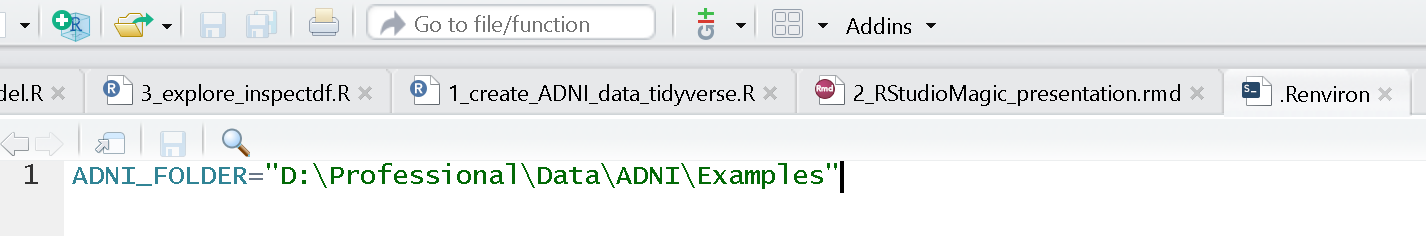
\includegraphics[width=0.8\textwidth,height=\textheight]{../external/images/setup_3_rstudio_project_environ2.PNG}
\end{itemize}

\end{frame}

\begin{frame}{Organize your project folders and markdown}
\protect\hypertarget{organize-your-project-folders-and-markdown}{}

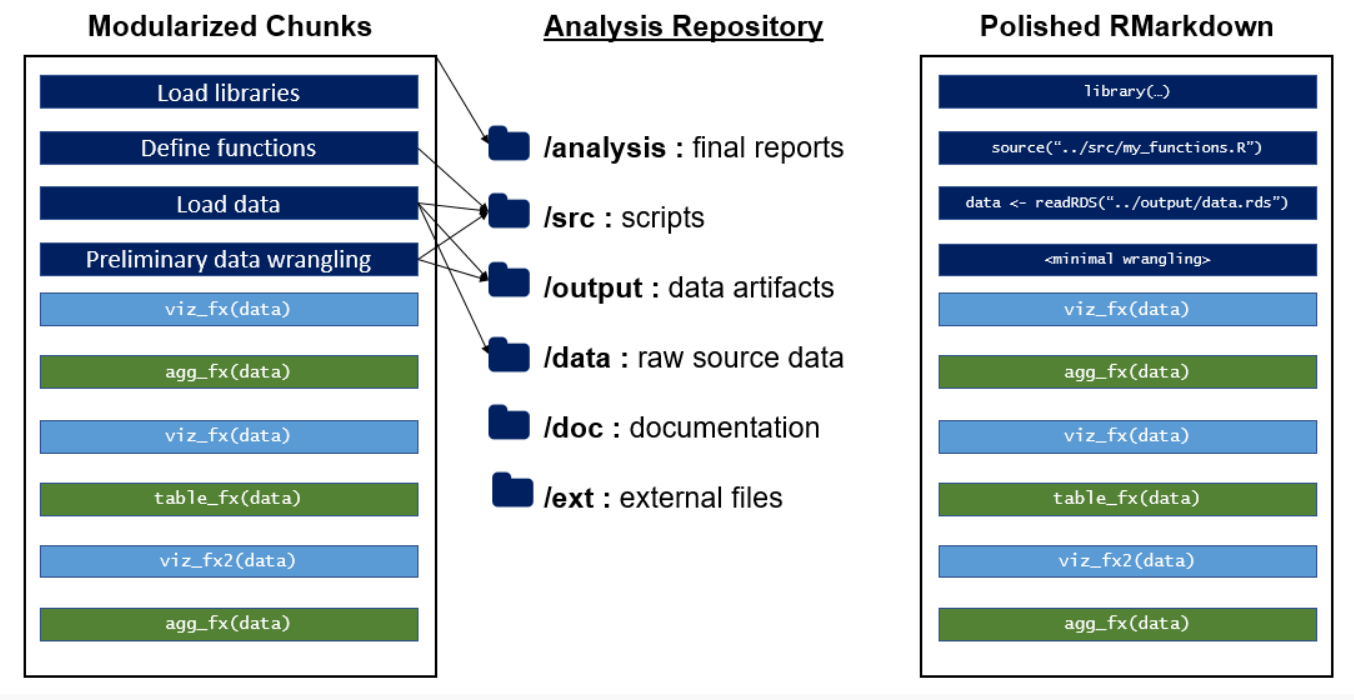
\includegraphics{../external/images/setup_4_markdown_project.PNG}

\url{https://emilyriederer.netlify.com/post/rmarkdown-driven-development/}

\end{frame}

\begin{frame}{Organize your project folders and markdown}
\protect\hypertarget{organize-your-project-folders-and-markdown-1}{}

\begin{itemize}
\tightlist
\item
  What works for you?
\item
  What works for your organization or team?
\item
  Maximize utility, minimize complexity
\end{itemize}

\end{frame}

\begin{frame}{This works for us}
\protect\hypertarget{this-works-for-us}{}

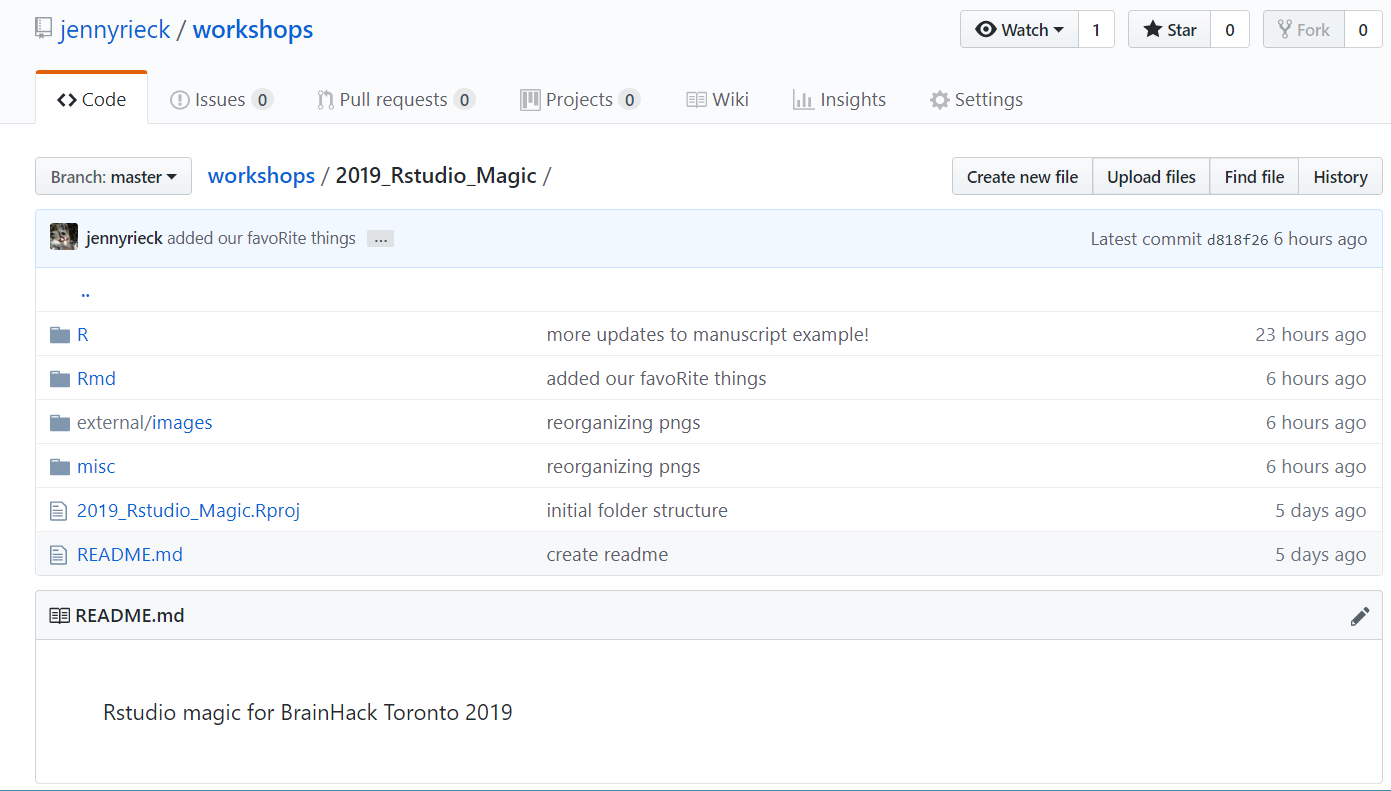
\includegraphics{../external/images/setup_5_git.PNG}

\end{frame}

\begin{frame}{This works for us}
\protect\hypertarget{this-works-for-us-1}{}

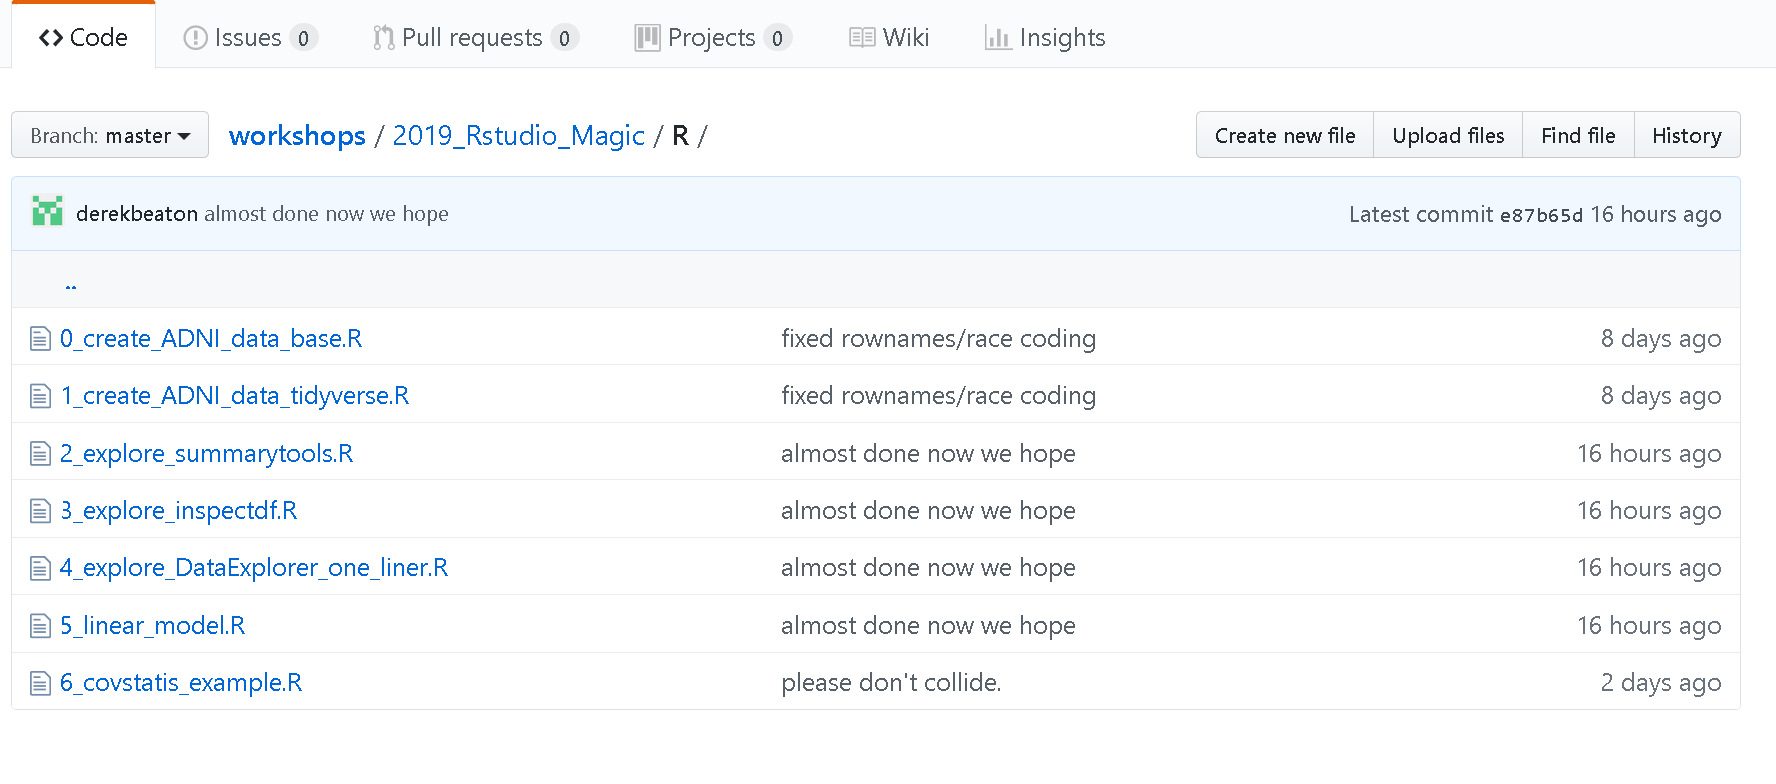
\includegraphics{../external/images/Rfolder.PNG}

\end{frame}

\begin{frame}{This works for us}
\protect\hypertarget{this-works-for-us-2}{}

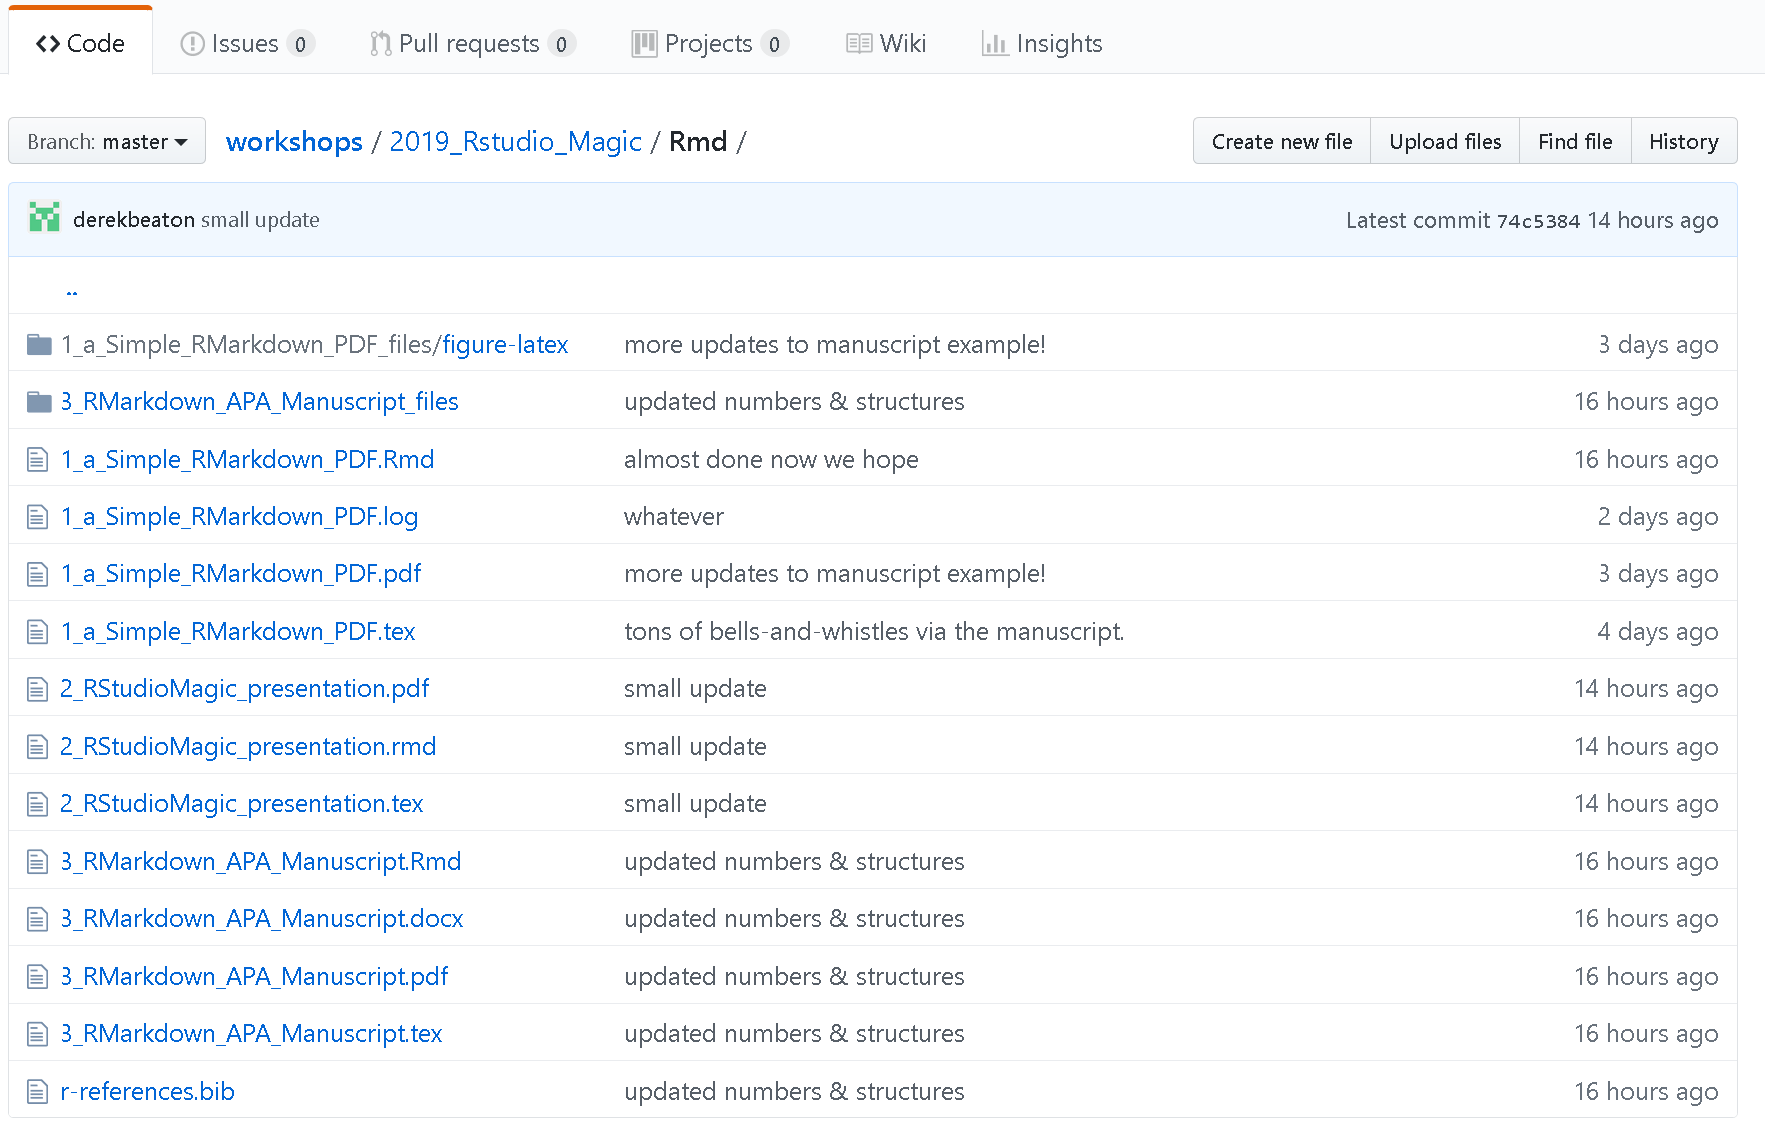
\includegraphics{../external/images/RMDfolder.PNG}

\end{frame}

\begin{frame}[fragile]{Get the packages you need}
\protect\hypertarget{get-the-packages-you-need}{}

e.g.,

\begin{Shaded}
\begin{Highlighting}[]
\CommentTok{#to install from CRAN}
\KeywordTok{install.pacakges}\NormalTok{(}\StringTok{'devtools'}\NormalTok{, }\DataTypeTok{depenedencies =} \OtherTok{TRUE}\NormalTok{)}

\CommentTok{#to install from a git  (requires the devtools package)}
\NormalTok{devtools}\OperatorTok{::}\KeywordTok{install_github}\NormalTok{(Gibbsdavidl}\OperatorTok{/}\NormalTok{CatterPlots)}

\CommentTok{#to install from a file}
\KeywordTok{install.packages}\NormalTok{(}\StringTok{'/mypath/to/package/ADNIMERGE.tar.gz'}\NormalTok{, }
                 \DataTypeTok{type=}\StringTok{'source'}\NormalTok{, }\DataTypeTok{repos=}\OtherTok{NULL}\NormalTok{) }
\end{Highlighting}
\end{Shaded}

(hint: you'll need more than this!)

\end{frame}

\hypertarget{part-3-r}{%
\section{Part 3: R}\label{part-3-r}}

\begin{frame}[fragile]{Let's take a closer look at R}
\protect\hypertarget{lets-take-a-closer-look-at-r}{}

\begin{itemize}
\tightlist
\item
  The Alzheimer's Disease Neuroimaging Initiative (ADNI).
\item
  We use the \texttt{ADNIMERGE} R package

  \begin{itemize}
  \tightlist
  \item
    Lots and lots of data prepared \emph{for you}
  \end{itemize}
\item
  We use this for all of our examples
\end{itemize}

\end{frame}

\begin{frame}[fragile]{The R examples}
\protect\hypertarget{the-r-examples}{}

\begin{itemize}
\tightlist
\item
  Making \& prepping data

  \begin{itemize}
  \tightlist
  \item
    \texttt{0\_create\_ADNI\_data\_base.R}
  \item
    \texttt{1\_create\_ADNI\_data\_tidyverse.R}
  \end{itemize}
\item
  Exploring data

  \begin{itemize}
  \tightlist
  \item
    \texttt{2\_explore\_summarytools.R}
  \item
    \texttt{3\_explore\_inspectdf.R}
  \item
    \texttt{4\_explore\_DataExplorer\_one\_liner.R}
  \item
    With a small rant from Derek
  \end{itemize}
\item
  Some stats: Linear models

  \begin{itemize}
  \tightlist
  \item
    \texttt{5\_linear\_model.R}
  \end{itemize}
\item
  Experimental packages (covSTATIS via Github)

  \begin{itemize}
  \tightlist
  \item
    \texttt{6\_covstatis\_example.R}
  \end{itemize}
\end{itemize}

\end{frame}

\begin{frame}{Derek's rant break}
\protect\hypertarget{dereks-rant-break}{}

\begin{itemize}
\tightlist
\item
  DataExplorer committed a crime.

  \begin{itemize}
  \tightlist
  \item
    ``coding categorical variables with the indicator matrix of dummy
    variables and considering them as Gaussian, for instance, is almost
    a crime.''
  \end{itemize}
\item
  See
  \href{https://github.com/derekbeaton/Workshops/tree/master/RTC/PCA_MCA_Resampling/}{Derek's
  PCA \& multiple correspondence analysis workshop}

  \begin{itemize}
  \tightlist
  \item
    Same data as this workshop
  \item
    All in R \& RMarkdown
  \end{itemize}
\end{itemize}

\end{frame}

\hypertarget{part-4-rmarkdown-more}{%
\section{Part 4: RMarkdown \& more}\label{part-4-rmarkdown-more}}

\begin{frame}[fragile]{RMarkdown}
\protect\hypertarget{rmarkdown}{}

\begin{itemize}
\tightlist
\item
  Yuhui Xie:

  \begin{itemize}
  \tightlist
  \item
    \url{https://bookdown.org/yihui/rmarkdown/}
  \end{itemize}
\item
  What it is \& why to use it
\item
  Fancy helpers:

  \begin{itemize}
  \tightlist
  \item
    \texttt{kable} \& \texttt{kableExtra}
  \item
    \texttt{grid} \& \texttt{gridExtra}
  \end{itemize}
\item
  Deviations for:

  \begin{itemize}
  \tightlist
  \item
    \texttt{LaTeX}
  \item
    \texttt{Python}
  \end{itemize}
\item
  Tying it all together through here
\end{itemize}

\end{frame}

\begin{frame}[fragile]{RMarkdown Don'ts}
\protect\hypertarget{rmarkdown-donts}{}

\begin{itemize}
\tightlist
\item
  Don't hardcode values or absolute file paths

  \begin{itemize}
  \tightlist
  \item
    see \texttt{here::here()}
  \item
    Use projects (\texttt{.Rproj})
  \end{itemize}
\item
  Don't do complicated or expensive stuff

  \begin{itemize}
  \tightlist
  \item
    Database queries
  \item
    Resampling
  \end{itemize}
\item
  avoid \texttt{eval=FALSE}

  \begin{itemize}
  \tightlist
  \item
    except to help illustrate code\ldots{}
  \end{itemize}
\item
  Reduce repeated code

  \begin{itemize}
  \tightlist
  \item
    One time: Script
  \item
    Two times: Function
  \item
    Three times: Package
  \end{itemize}
\end{itemize}

\end{frame}

\begin{frame}{RMarkdown dos \& don'ts}
\protect\hypertarget{rmarkdown-dos-donts}{}

\begin{itemize}
\tightlist
\item
  Suggestions \& More:

  \begin{itemize}
  \tightlist
  \item
    \url{https://emilyriederer.netlify.com/post/rmarkdown-driven-development/}
  \end{itemize}
\item
  We're using this here
\end{itemize}

\end{frame}

\begin{frame}[fragile]{Let's take a look}
\protect\hypertarget{lets-take-a-look}{}

\begin{itemize}
\tightlist
\item
  \texttt{1\_a\_Simple\_RMarkdown\_PDF.Rmd}
\item
  \texttt{2\_RStudioMagic\_presentation.rmd}

  \begin{itemize}
  \tightlist
  \item
    This presentation!
  \end{itemize}
\item
  \texttt{3\_RMarkdown\_APA\_Manuscript.Rmd}
\end{itemize}

\end{frame}

\hypertarget{part-5-advanced-topics}{%
\section{Part 5: ``Advanced'' topics}\label{part-5-advanced-topics}}

\begin{frame}{Some advanced/other things we're not covering}
\protect\hypertarget{some-advancedother-things-were-not-covering}{}

\begin{itemize}
\tightlist
\item
  package development
\item
  Shiny
\item
  SQL
\item
  C/C++
\item
  R2D3 (JavaScript)
\end{itemize}

\end{frame}

\begin{frame}{A few of our favorite things}
\protect\hypertarget{a-few-of-our-favorite-things}{}

\begin{itemize}
\tightlist
\item
  Fun R do-dads
\end{itemize}

\end{frame}

\begin{frame}[fragile]{CatterPlot for feline based graphics:}
\protect\hypertarget{catterplot-for-feline-based-graphics}{}

\texttt{devtools::install\_github(Gibbsdavidl/CatterPlots)}

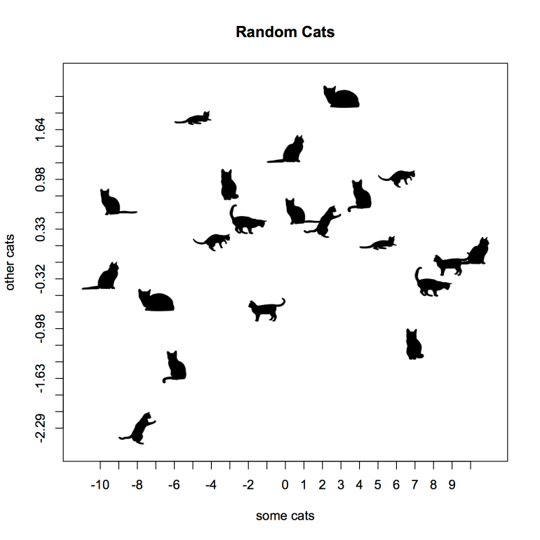
\includegraphics[width=0.6\textwidth,height=\textheight]{../external/images/funR_1_catterplotter.png}

\url{https://github.com/Gibbsdavidl/CatterPlots}

\end{frame}

\begin{frame}[fragile]{What's a pirate's favorite programming language?}
\protect\hypertarget{whats-a-pirates-favorite-programming-language}{}

\texttt{install.packages(\textquotesingle{}yarrr\textquotesingle{})}

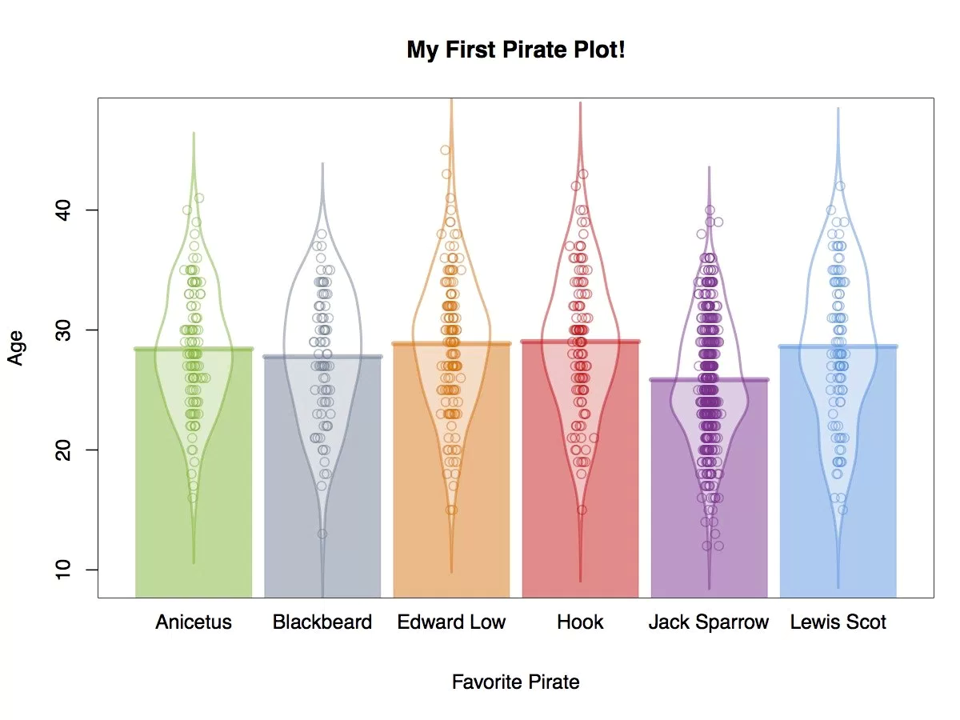
\includegraphics[width=0.75\textwidth,height=\textheight]{../external/images/funR_2_pirate.png}

\url{https://cran.r-project.org/web/packages/yarrr/vignettes/pirateplot.html}

\end{frame}

\begin{frame}[fragile]{Color palettes to fit your mood}
\protect\hypertarget{color-palettes-to-fit-your-mood}{}

\texttt{devtools::install\_github(karthik/wesanderson)}

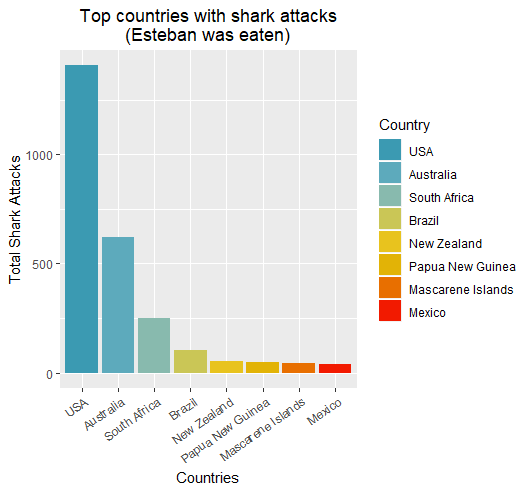
\includegraphics[width=0.6\textwidth,height=\textheight]{../external/images/funR_3_wes_anderson.png}

\url{https://github.com/karthik/wesanderson}

\end{frame}

\begin{frame}[fragile]{Mapping your Strava routes}
\protect\hypertarget{mapping-your-strava-routes}{}

\texttt{devtools::install\_github(marcusvolz/strava)}

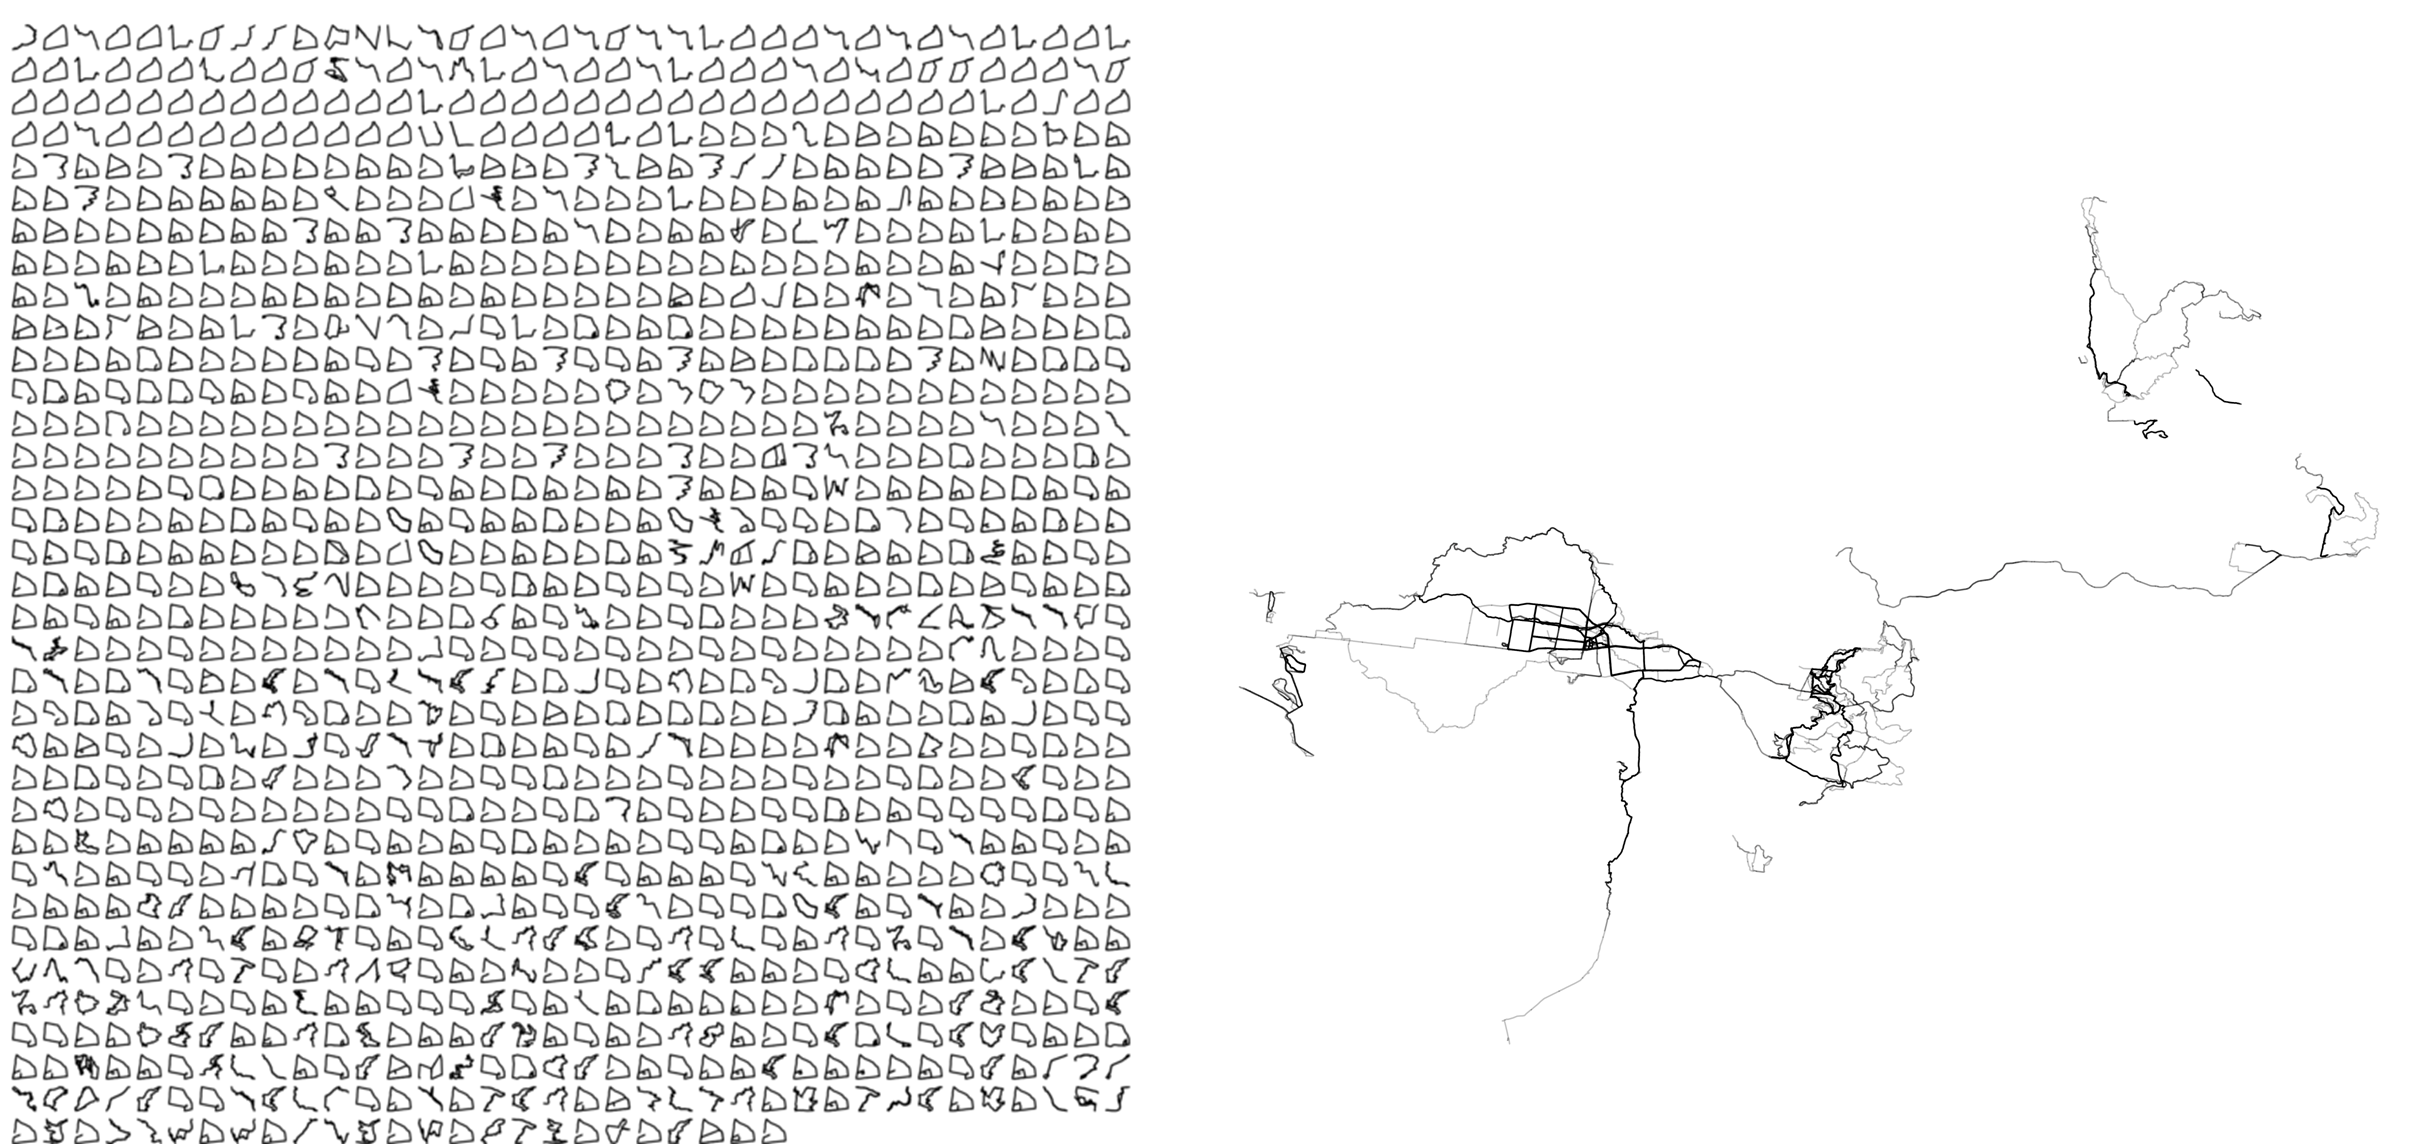
\includegraphics{../external/images/funR_4_strava_combo.png}

\url{https://www.r-bloggers.com/strava-rides-map-in-r/}

ALSO \url{https://marcusvolz.com/?p=4068}

\end{frame}

\begin{frame}{Make aRt!}
\protect\hypertarget{make-art}{}

\begin{itemize}
\tightlist
\item
  R Graph Gallery

  \begin{itemize}
  \tightlist
  \item
    \url{http://www.r-graph-gallery.com/}
  \end{itemize}
\item
  Rtist: Gaston Sanchez

  \begin{itemize}
  \tightlist
  \item
    \url{http://gastonsanchez.com/Rtist/}
  \end{itemize}
\end{itemize}

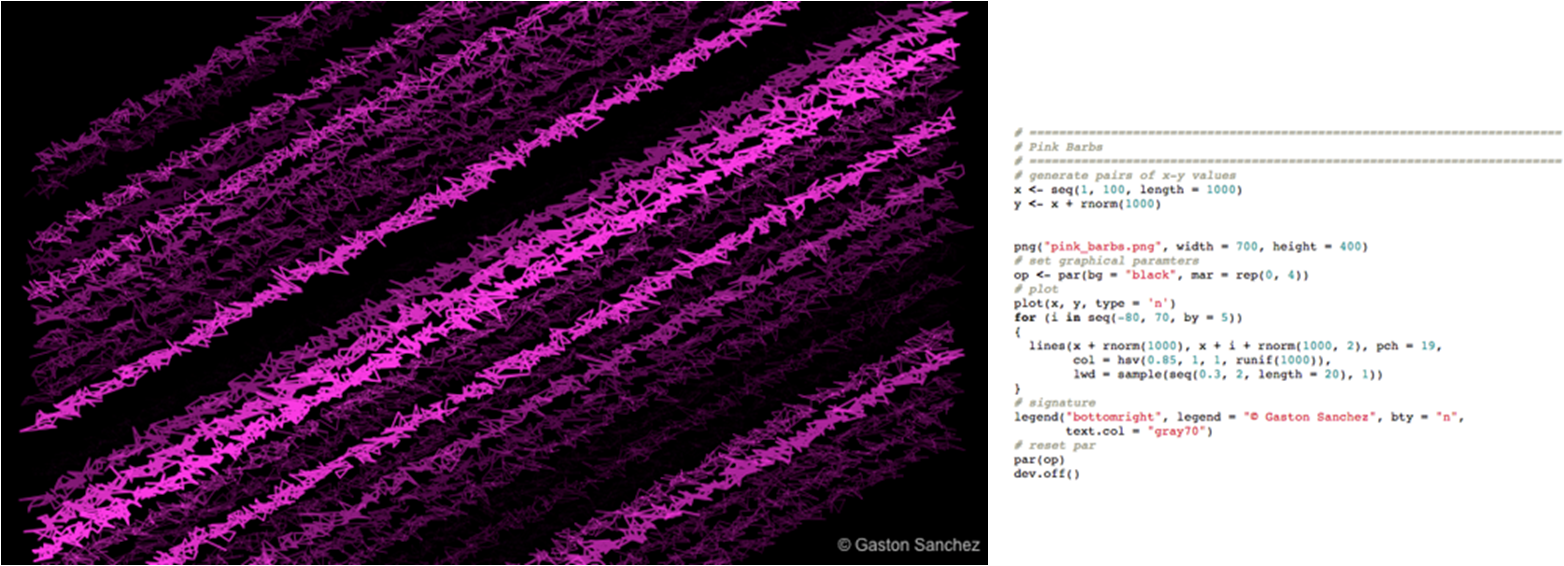
\includegraphics{../external/images/funR_5_aRt_pink_combo.png}

\end{frame}

\begin{frame}{Wouldn't be a brain hack without brains}
\protect\hypertarget{wouldnt-be-a-brain-hack-without-brains}{}

\end{frame}

\begin{frame}{R \& Brain Imaging}
\protect\hypertarget{r-brain-imaging}{}

\begin{itemize}
\tightlist
\item
  Slow to take hold

  \begin{itemize}
  \tightlist
  \item
    Getting there
  \end{itemize}
\item
  Neuroimaging: one of the last fields in R

  \begin{itemize}
  \tightlist
  \item
    Virtually every other field has an R community
  \item
    Bioinformatics especially (see
    \href{https://www.bioconductor.org/}{Bioconductor})
  \end{itemize}
\end{itemize}

\end{frame}

\begin{frame}[fragile]{Reading \& manipulating}
\protect\hypertarget{reading-manipulating}{}

\begin{itemize}
\tightlist
\item
  The neuroimaging ecosystem is growing in R

  \begin{itemize}
  \tightlist
  \item
    \texttt{neuroim}
  \item
    \texttt{ANTsR}
  \item
    \texttt{oro.nifti} - been around a while
  \item
    \texttt{RMINC}
  \end{itemize}
\end{itemize}

\end{frame}

\begin{frame}{More brains}
\protect\hypertarget{more-brains}{}

\begin{itemize}
\tightlist
\item
  \href{https://community.rstudio.com/t/shiny-contest-submission-shinymri-view-mri-images-in-shiny/23995}{MRI
  in Shiny}
\item
  \href{https://github.com/cwatson/brainGraph}{brainGraph}
\item
  \href{https://github.com/LCBC-UiO/ggseg}{ggSeg}
\end{itemize}


\includegraphics[width=0.4\textwidth,height=\textheight]{../external/images/ggseglogo.png}

\end{frame}

\begin{frame}{Neuroconductor}
\protect\hypertarget{neuroconductor}{}

\begin{itemize}
\tightlist
\item
  Conceptually based on Bioconductor
\item
  \url{https://neuroconductor.org/}
\end{itemize}


\includegraphics[width=0.4\textwidth,height=\textheight]{../external/images/neuro_logo1.png}

\end{frame}

\end{document}
